%%=============================================================================
%% LaTeX sjabloon voor bachelorproef, HoGent Bedrijf en Organisatie
%% Opleiding Toegepaste Informatica
%%=============================================================================

\documentclass[fleqn,a4paper,12pt]{book}

%%=============================================================================
%% LaTeX sjabloon voor de bachelorproef, HoGent Bedrijf en Organisatie
%% Opleiding toegepaste informatica
%%
%% Structuur en algemene vormgeving. Meestal hoef je hier niets te wijzigen.
%%
%% Vormgeving gebaseerd op "The Legrand Orange Book", version 2.0 (9/2/15)
%% door Mathias Legrand (legrand.mathias@gmail.com) met aanpassingen door
%% Vel (vel@latextemplates.com). Het oorspronkelijke template is te vinden op
%% http://www.LaTeXTemplates.com
%%
%% Aanpassingen voor HoGent toegepaste informatica: 
%%   Bert Van Vreckem <bert.vanvreckem@hogent.be>
%% Licentie: 
%%   CC BY-NC-SA 3.0 (http://creativecommons.org/licenses/by-nc-sa/3.0/)
%%=============================================================================

%%-----------------------------------------------------------------------------
%% Packages
%%-----------------------------------------------------------------------------

\usepackage[top=3cm,bottom=3cm,left=3cm,right=3cm,headsep=10pt,a4paper]{geometry} % Page margins
\usepackage[utf8]{inputenc}  % Accenten gebruiken in tekst (vb. é ipv \'e)
\usepackage{amsfonts}        % AMS math packages: extra wiskundige
\usepackage{amsmath}         %   symbolen (o.a. getallen-
\usepackage{amssymb}         %   verzamelingen N, R, Z, Q, etc.)
\usepackage[english,dutch]{babel}    % Taalinstellingen: woordsplitsingen,
                             %  commando's voor speciale karakters
                             %  ("dutch" voor NL)
                             

\usepackage{listings}
\usepackage{iflang}
\usepackage{eurosym}         % Euro-symbool €
\usepackage{geometry}
\usepackage{graphicx}        % Invoegen van tekeningen
\graphicspath{{img/}}       % Specifies the directory where pictures are stored
\usepackage{tikz}            % Required for drawing custom shapes
\usepackage[pdftex,bookmarks=true]{hyperref}
\usepackage{titlesec}
\usepackage[most]{tcolorbox}
                             % PDF krijgt klikbare links & verwijzingen,
                             %  inhoudstafel
\usepackage{enumitem}        % Customize lists
\setlist{nolistsep}         % Reduce spacing between list items
\usepackage{listings}        % Broncode mooi opmaken
\usepackage{multirow}        % Tekst over verschillende cellen in tabellen
\usepackage{rotating}        % Tabellen en figuren roteren

\usepackage{booktabs}        % Required for nicer horizontal rules in tables

\usepackage{xcolor}          % Required for specifying colors by name
\definecolor{maincolor}{RGB}{0,147,208} % Define the main color used for 
                             % highlighting throughout the book
                             % 0, 147, 208 = officiële kleur HoGent FBO
\newtcblisting{cisco}[1][]{size=fbox, listing only, listing options={style=tcblatex,basicstyle=\ttfamily\scriptsize,tabsize=2,language=sh},#1}

% Paragraph style: no indent, add space between paragraphs
\setlength{\parindent}{0em}
\setlength{\parskip}{1em}

\usepackage{etoolbox}
\usepackage{titling} % Macros for title, author, etc
\usepackage{lipsum}          % Voor vultekst (lorem ipsum)

%----------------------------------------------------------------------------------------
%	FONTS
%----------------------------------------------------------------------------------------

\usepackage{avant} % Use the Avantgarde font for headings
%\usepackage{times} % Use the Times font for headings
\usepackage{mathptmx} % Use the Adobe Times Roman as the default text font together with math symbols from the Sym­bol, Chancery and Com­puter Modern fonts

\usepackage{microtype} % Slightly tweak font spacing for aesthetics
\usepackage[utf8]{inputenc} % Required for including letters with accents
\usepackage[T1]{fontenc} % Use 8-bit encoding that has 256 glyphs

%------------------------------------------------------------------------------
%	TITLE PAGE
%------------------------------------------------------------------------------

\newcommand{\inserttitlepage}{%
\begin{titlepage}
  \newgeometry{top=2cm,bottom=1.5cm,left=1.5cm,right=1.5cm}
  \begin{center}

    \begingroup
    \rmfamily
    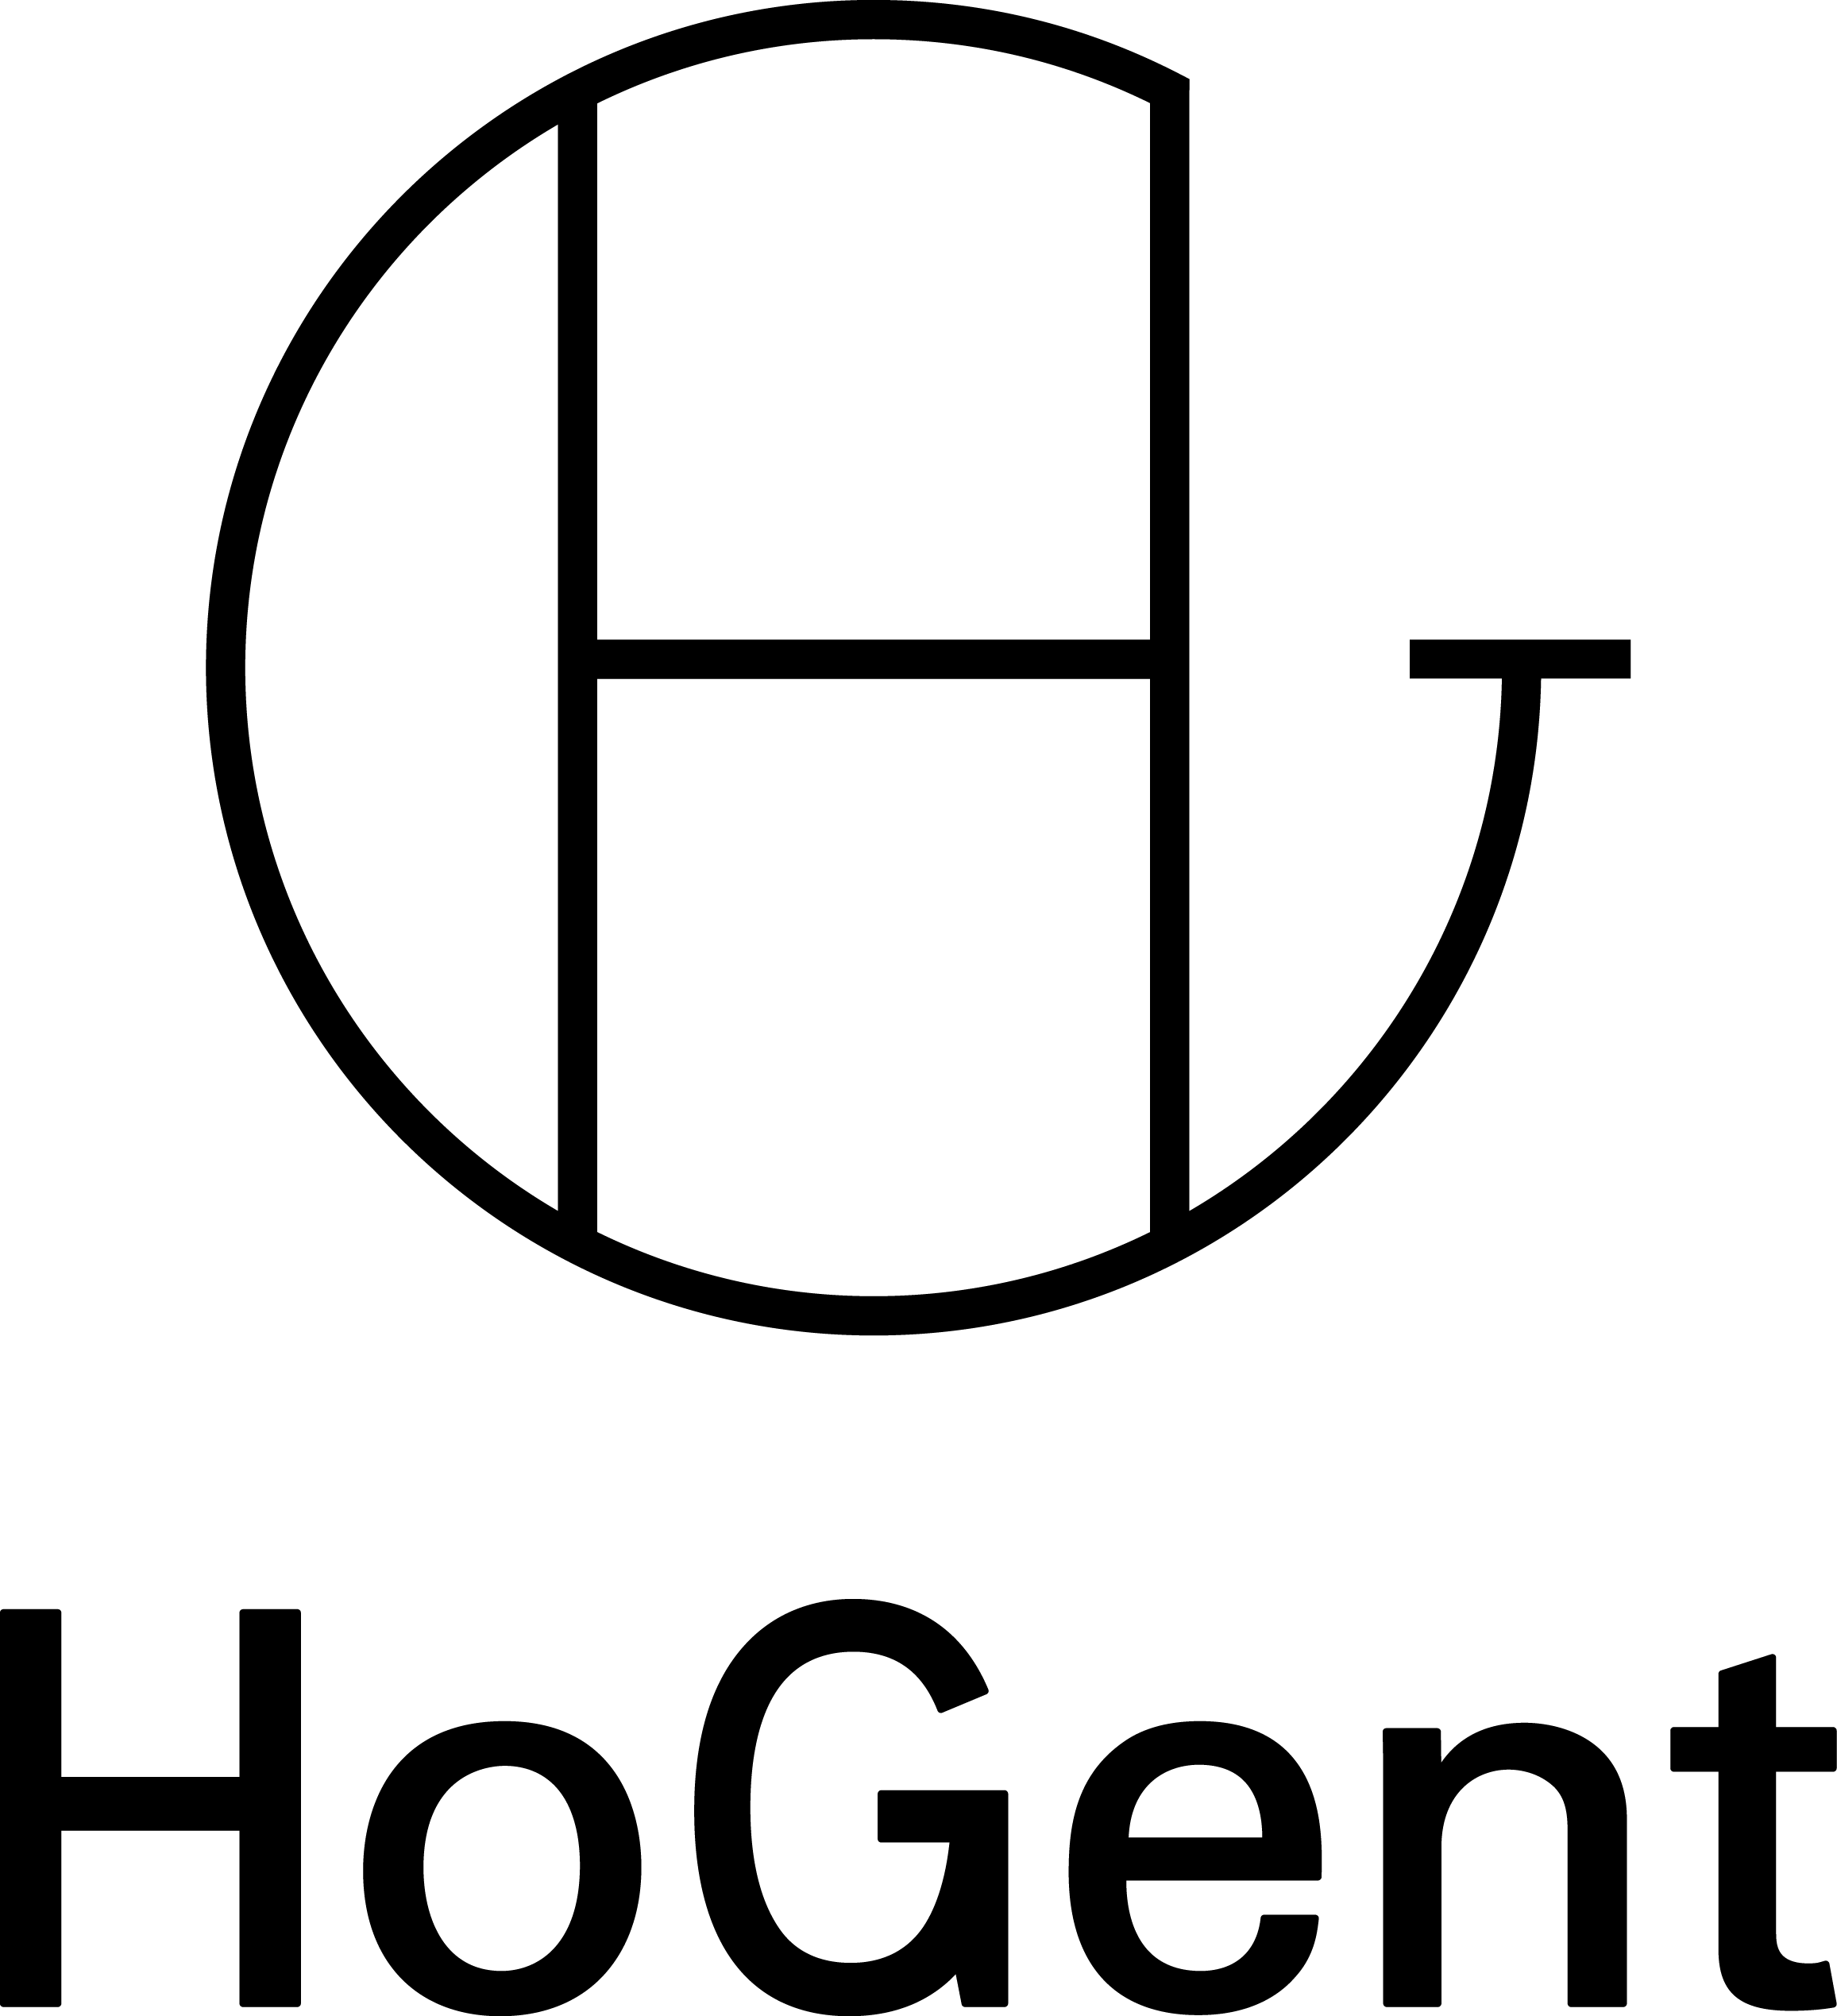
\includegraphics[width=2.5cm]{img/HG-beeldmerk-woordmerk}\\[.5cm]
    Faculteit Bedrijf en Organisatie\\[3cm]
    \titel
    \vfill
    \student\\[3.5cm]
    Scriptie voorgedragen tot het bekomen van de graad van\\professionele bachelor in de toegepaste informatica\\[2cm]
    Promotor:\\
    \promotor\\
    \ifdefempty{\copromotor}{\vspace{2.5cm}}{Co-promotor:\\\copromotor\\[2.5cm]}
    Instelling: \instelling\\[.5cm]
    Academiejaar: \academiejaar\\[.5cm]
    \ifcase \examenperiode \or Eerste \or Tweede \else Derde \fi examenperiode
    \endgroup

  \end{center}
  \restoregeometry
\end{titlepage}
  \emptypage
\begin{titlepage}
  \newgeometry{top=5.35cm,bottom=1.5cm,left=1.5cm,right=1.5cm}
  \begin{center}

    \begingroup
    \rmfamily
    \IfLanguageName{dutch}{Faculteit Bedrijf en Organisatie}{Faculty of Business and Information Management}\\[3cm]
    \titel
    \vfill
    \student\\[3.5cm]
    \IfLanguageName{dutch}{Scriptie voorgedragen tot het bekomen van de graad van\\professionele bachelor in de toegepaste informatica}{Thesis submitted in partial fulfilment of the requirements for the degree of\\professional bachelor of applied computer science}\\[2cm]
    Promotor:\\
    \promotor\\
    \ifdefempty{\copromotor}{\vspace{2.5cm}}{Co-promotor:\\\copromotor\\[2.5cm]}
    \IfLanguageName{dutch}{Instelling}{Institution}: \instelling\\[.5cm]
    \IfLanguageName{dutch}{Academiejaar}{Academic year}: \academiejaar\\[.5cm]
    \IfLanguageName{dutch}{%
    \ifcase \examenperiode \or Eerste \or Tweede \else Derde \fi examenperiode}{%
    \ifcase \examenperiode \or First \or Second \else Third \fi examination period}
    \endgroup

  \end{center}
  \restoregeometry
\end{titlepage}
}

%----------------------------------------------------------------------------------------
%	BIBLIOGRAPHY AND INDEX
%----------------------------------------------------------------------------------------

\usepackage[style=apa,backend=biber]{biblatex}
\usepackage{csquotes}
\DeclareLanguageMapping{dutch}{dutch-apa}
\addbibresource{bachproef-tin.bib} % BibTeX bibliography file
\addbibresource{../voorstel/voorstel.bib}
\defbibheading{bibempty}{}

\usepackage{calc} % For simpler calculation - used for spacing the index letter headings correctly
\usepackage{makeidx} % Required to make an index
\makeindex % Tells LaTeX to create the files required for indexing

%----------------------------------------------------------------------------------------
%	MAIN TABLE OF CONTENTS
%----------------------------------------------------------------------------------------

\usepackage{titletoc} % Required for manipulating the table of contents

\contentsmargin{0cm} % Removes the default margin

% Part text styling
\titlecontents{part}[0cm]
{\addvspace{20pt}\centering\large\bfseries}
{}
{}
{}

% Chapter text styling
\titlecontents{chapter}[1.25cm] % Indentation
{\addvspace{12pt}\large\sffamily\bfseries} % Spacing and font options for chapters
{\color{maincolor!60}\contentslabel[\Large\thecontentslabel]{1.25cm}\color{maincolor}} % Chapter number
{\color{maincolor}}
{\color{maincolor!60}\normalsize\;\titlerule*[.5pc]{.}\;\thecontentspage} % Page number

% Section text styling
\titlecontents{section}[1.25cm] % Indentation
{\addvspace{3pt}\sffamily\bfseries} % Spacing and font options for sections
{\contentslabel[\thecontentslabel]{1.25cm}} % Section number
{}
{\hfill\color{black}\thecontentspage} % Page number
[]

% Subsection text styling
\titlecontents{subsection}[1.25cm] % Indentation
{\addvspace{1pt}\sffamily\small} % Spacing and font options for subsections
{\contentslabel[\thecontentslabel]{1.25cm}} % Subsection number
{}
{\ \titlerule*[.5pc]{.}\;\thecontentspage} % Page number
[]

% List of figures
\titlecontents{figure}[0em]
{\addvspace{-5pt}\sffamily}
{\thecontentslabel\hspace*{1em}}
{}
{\ \titlerule*[.5pc]{.}\;\thecontentspage}
[]

% List of tables
\titlecontents{table}[0em]
{\addvspace{-5pt}\sffamily}
{\thecontentslabel\hspace*{1em}}
{}
{\ \titlerule*[.5pc]{.}\;\thecontentspage}
[]

%----------------------------------------------------------------------------------------
%	MINI TABLE OF CONTENTS IN PART HEADS
%----------------------------------------------------------------------------------------

% Chapter text styling
\titlecontents{lchapter}[0em] % Indenting
{\addvspace{15pt}\large\sffamily\bfseries} % Spacing and font options for chapters
{\color{maincolor}\contentslabel[\Large\thecontentslabel]{1.25cm}\color{maincolor}} % Chapter number
{}
{\color{maincolor}\normalsize\sffamily\bfseries\;\titlerule*[.5pc]{.}\;\thecontentspage} % Page number

% Section text styling
\titlecontents{lsection}[0em] % Indenting
{\sffamily\small} % Spacing and font options for sections
{\contentslabel[\thecontentslabel]{1.25cm}} % Section number
{}
{}

% Subsection text styling
\titlecontents{lsubsection}[.5em] % Indentation
{\normalfont\footnotesize\sffamily} % Font settings
{}
{}
{}

%----------------------------------------------------------------------------------------
%	PAGE HEADERS
%----------------------------------------------------------------------------------------

\usepackage{fancyhdr} % Required for header and footer configuration

\pagestyle{fancy}
\renewcommand{\chaptermark}[1]{\markboth{\sffamily\normalsize\bfseries\chaptername\ \thechapter.\ #1}{}} % Chapter text font settings
\renewcommand{\sectionmark}[1]{\markright{\sffamily\normalsize\thesection\hspace{5pt}#1}{}} % Section text font settings
\fancyhf{} \fancyhead[LE,RO]{\sffamily\normalsize\thepage} % Font setting for the page number in the header
\fancyhead[LO]{\rightmark} % Print the nearest section name on the left side of odd pages
\fancyhead[RE]{\leftmark} % Print the current chapter name on the right side of even pages
\renewcommand{\headrulewidth}{0.5pt} % Width of the rule under the header
\addtolength{\headheight}{2.5pt} % Increase the spacing around the header slightly
\renewcommand{\footrulewidth}{0pt} % Removes the rule in the footer
\fancypagestyle{plain}{\fancyhead{}\renewcommand{\headrulewidth}{0pt}} % Style for when a plain pagestyle is specified

% Removes the header from odd empty pages at the end of chapters
\makeatletter
\renewcommand{\cleardoublepage}{
\clearpage\ifodd\c@page\else
\hbox{}
\vspace*{\fill}
\thispagestyle{empty}
\newpage
\fi}

%----------------------------------------------------------------------------------------
%	THEOREM STYLES
%----------------------------------------------------------------------------------------

\usepackage{amsmath,amsfonts,amssymb,amsthm} % For math equations, theorems, symbols, etc

\newcommand{\intoo}[2]{\mathopen{]}#1\,;#2\mathclose{[}}
\newcommand{\ud}{\mathop{\mathrm{{}d}}\mathopen{}}
\newcommand{\intff}[2]{\mathopen{[}#1\,;#2\mathclose{]}}
\newtheorem{notation}{Notation}[chapter]

% Boxed/framed environments
\newtheoremstyle{maincolornumbox}% % Theorem style name
{0pt}% Space above
{0pt}% Space below
{\normalfont}% % Body font
{}% Indent amount
{\small\bf\sffamily\color{maincolor}}% % Theorem head font
{\;}% Punctuation after theorem head
{0.25em}% Space after theorem head
{\small\sffamily\color{maincolor}\thmname{#1}\nobreakspace\thmnumber{\@ifnotempty{#1}{}\@upn{#2}}% Theorem text (e.g. Theorem 2.1)
\thmnote{\nobreakspace\the\thm@notefont\sffamily\bfseries\color{black}---\nobreakspace#3.}} % Optional theorem note
\renewcommand{\qedsymbol}{$\blacksquare$}% Optional qed square

\newtheoremstyle{blacknumex}% Theorem style name
{5pt}% Space above
{5pt}% Space below
{\normalfont}% Body font
{} % Indent amount
{\small\bf\sffamily}% Theorem head font
{\;}% Punctuation after theorem head
{0.25em}% Space after theorem head
{\small\sffamily{\tiny\ensuremath{\blacksquare}}\nobreakspace\thmname{#1}\nobreakspace\thmnumber{\@ifnotempty{#1}{}\@upn{#2}}% Theorem text (e.g. Theorem 2.1)
\thmnote{\nobreakspace\the\thm@notefont\sffamily\bfseries---\nobreakspace#3.}}% Optional theorem note

\newtheoremstyle{blacknumbox} % Theorem style name
{0pt}% Space above
{0pt}% Space below
{\normalfont}% Body font
{}% Indent amount
{\small\bf\sffamily}% Theorem head font
{\;}% Punctuation after theorem head
{0.25em}% Space after theorem head
{\small\sffamily\thmname{#1}\nobreakspace\thmnumber{\@ifnotempty{#1}{}\@upn{#2}}% Theorem text (e.g. Theorem 2.1)
\thmnote{\nobreakspace\the\thm@notefont\sffamily\bfseries---\nobreakspace#3.}}% Optional theorem note

% Non-boxed/non-framed environments
\newtheoremstyle{maincolornum}% % Theorem style name
{5pt}% Space above
{5pt}% Space below
{\normalfont}% % Body font
{}% Indent amount
{\small\bf\sffamily\color{maincolor}}% % Theorem head font
{\;}% Punctuation after theorem head
{0.25em}% Space after theorem head
{\small\sffamily\color{maincolor}\thmname{#1}\nobreakspace\thmnumber{\@ifnotempty{#1}{}\@upn{#2}}% Theorem text (e.g. Theorem 2.1)
\thmnote{\nobreakspace\the\thm@notefont\sffamily\bfseries\color{black}---\nobreakspace#3.}} % Optional theorem note
\renewcommand{\qedsymbol}{$\blacksquare$}% Optional qed square
\makeatother

% Defines the theorem text style for each type of theorem to one of the three styles above
\newcounter{dummy}
\numberwithin{dummy}{section}
\theoremstyle{maincolornumbox}
\newtheorem{theoremeT}[dummy]{Theorem}
\newtheorem{problem}{Problem}[chapter]
\newtheorem{exerciseT}{Exercise}[chapter]
\theoremstyle{blacknumex}
\newtheorem{exampleT}{Example}[chapter]
\theoremstyle{blacknumbox}
\newtheorem{vocabulary}{Vocabulary}[chapter]
\newtheorem{definitionT}{Definition}[section]
\newtheorem{corollaryT}[dummy]{Corollary}
\theoremstyle{maincolornum}
\newtheorem{proposition}[dummy]{Proposition}

%----------------------------------------------------------------------------------------
%	DEFINITION OF COLORED BOXES
%----------------------------------------------------------------------------------------

\RequirePackage[framemethod=default]{mdframed} % Required for creating the theorem, definition, exercise and corollary boxes

% Theorem box
\newmdenv[skipabove=7pt,
skipbelow=7pt,
backgroundcolor=black!5,
linecolor=maincolor,
innerleftmargin=5pt,
innerrightmargin=5pt,
innertopmargin=5pt,
leftmargin=0cm,
rightmargin=0cm,
innerbottommargin=5pt]{tBox}

% Exercise box
\newmdenv[skipabove=7pt,
skipbelow=7pt,
rightline=false,
leftline=true,
topline=false,
bottomline=false,
backgroundcolor=maincolor!10,
linecolor=maincolor,
innerleftmargin=5pt,
innerrightmargin=5pt,
innertopmargin=5pt,
innerbottommargin=5pt,
leftmargin=0cm,
rightmargin=0cm,
linewidth=4pt]{eBox}

% Definition box
\newmdenv[skipabove=7pt,
skipbelow=7pt,
rightline=false,
leftline=true,
topline=false,
bottomline=false,
linecolor=maincolor,
innerleftmargin=5pt,
innerrightmargin=5pt,
innertopmargin=0pt,
leftmargin=0cm,
rightmargin=0cm,
linewidth=4pt,
innerbottommargin=0pt]{dBox}

% Corollary box
\newmdenv[skipabove=7pt,
skipbelow=7pt,
rightline=false,
leftline=true,
topline=false,
bottomline=false,
linecolor=gray,
backgroundcolor=black!5,
innerleftmargin=5pt,
innerrightmargin=5pt,
innertopmargin=5pt,
leftmargin=0cm,
rightmargin=0cm,
linewidth=4pt,
innerbottommargin=5pt]{cBox}

% Creates an environment for each type of theorem and assigns it a theorem text style from the "Theorem Styles" section above and a colored box from above
\newenvironment{theorem}{\begin{tBox}\begin{theoremeT}}{\end{theoremeT}\end{tBox}}
\newenvironment{exercise}{\begin{eBox}\begin{exerciseT}}{\hfill{\color{maincolor}\tiny\ensuremath{\blacksquare}}\end{exerciseT}\end{eBox}}
\newenvironment{definition}{\begin{dBox}\begin{definitionT}}{\end{definitionT}\end{dBox}}
\newenvironment{example}{\begin{exampleT}}{\hfill{\tiny\ensuremath{\blacksquare}}\end{exampleT}}
\newenvironment{corollary}{\begin{cBox}\begin{corollaryT}}{\end{corollaryT}\end{cBox}}

%----------------------------------------------------------------------------------------
%	REMARK ENVIRONMENT
%----------------------------------------------------------------------------------------

\newenvironment{remark}{\par\vspace{10pt}\small % Vertical white space above the remark and smaller font size
\begin{list}{}{
\leftmargin=35pt % Indentation on the left
\rightmargin=25pt}\item\ignorespaces % Indentation on the right
\makebox[-2.5pt]{\begin{tikzpicture}[overlay]
\node[draw=maincolor!60,line width=1pt,circle,fill=maincolor!25,font=\sffamily\bfseries,inner sep=2pt,outer sep=0pt] at (-15pt,0pt){\textcolor{maincolor}{R}};\end{tikzpicture}} % Orange R in a circle
\advance\baselineskip -1pt}{\end{list}\vskip5pt} % Tighter line spacing and white space after remark

%----------------------------------------------------------------------------------------
%	SECTION NUMBERING IN THE MARGIN
%----------------------------------------------------------------------------------------

\makeatletter
\renewcommand{\@seccntformat}[1]{\llap{\textcolor{maincolor}{\csname the#1\endcsname}\hspace{1em}}}
\renewcommand{\section}{\@startsection{section}{1}{\z@}
{-4ex \@plus -1ex \@minus -.4ex}
{1ex \@plus.2ex }
{\normalfont\large\sffamily\bfseries}}
\renewcommand{\subsection}{\@startsection {subsection}{2}{\z@}
{-3ex \@plus -0.1ex \@minus -.4ex}
{0.5ex \@plus.2ex }
{\normalfont\sffamily\bfseries}}
\renewcommand{\subsubsection}{\@startsection {subsubsection}{3}{\z@}
{-2ex \@plus -0.1ex \@minus -.2ex}
{.2ex \@plus.2ex }
{\normalfont\small\sffamily\bfseries}}
\renewcommand\paragraph{\@startsection{paragraph}{4}{\z@}
{-2ex \@plus-.2ex \@minus .2ex}
{.1ex}
{\normalfont\small\sffamily\bfseries}}

%----------------------------------------------------------------------------------------
%	PART HEADINGS
%----------------------------------------------------------------------------------------

% numbered part in the table of contents
\newcommand{\@mypartnumtocformat}[2]{%
\setlength\fboxsep{0pt}%
\noindent\colorbox{maincolor!20}{\strut\parbox[c][.7cm]{\ecart}{\color{maincolor!70}\Large\sffamily\bfseries\centering#1}}\hskip\esp\colorbox{maincolor!40}{\strut\parbox[c][.7cm]{\linewidth-\ecart-\esp}{\Large\sffamily\centering#2}}}%
%%%%%%%%%%%%%%%%%%%%%%%%%%%%%%%%%%
% unnumbered part in the table of contents
\newcommand{\@myparttocformat}[1]{%
\setlength\fboxsep{0pt}%
\noindent\colorbox{maincolor!40}{\strut\parbox[c][.7cm]{\linewidth}{\Large\sffamily\centering#1}}}%
%%%%%%%%%%%%%%%%%%%%%%%%%%%%%%%%%%
\newlength\esp
\setlength\esp{4pt}
\newlength\ecart
\setlength\ecart{1.2cm-\esp}
\newcommand{\thepartimage}{}%
\newcommand{\partimage}[1]{\renewcommand{\thepartimage}{#1}}%
\def\@part[#1]#2{%
\ifnum \c@secnumdepth >-2\relax%
\refstepcounter{part}%
\addcontentsline{toc}{part}{\texorpdfstring{\protect\@mypartnumtocformat{\thepart}{#1}}{\partname~\thepart\ ---\ #1}}
\else%
\addcontentsline{toc}{part}{\texorpdfstring{\protect\@myparttocformat{#1}}{#1}}%
\fi%
\startcontents%
\markboth{}{}%
{\thispagestyle{empty}%
\begin{tikzpicture}[remember picture,overlay]%
\node at (current page.north west){\begin{tikzpicture}[remember picture,overlay]%
\fill[maincolor!20](0cm,0cm) rectangle (\paperwidth,-\paperheight);
\node[anchor=north] at (4cm,-3.25cm){\color{maincolor!40}\fontsize{220}{100}\sffamily\bfseries\@Roman\c@part};
\node[anchor=south east] at (\paperwidth-1cm,-\paperheight+1cm){\parbox[t][][t]{8.5cm}{
\printcontents{l}{0}{\setcounter{tocdepth}{1}}%
}};
\node[anchor=north east] at (\paperwidth-1.5cm,-3.25cm){\parbox[t][][t]{15cm}{\strut\raggedleft\color{white}\fontsize{30}{30}\sffamily\bfseries#2}};
\end{tikzpicture}};
\end{tikzpicture}}%
\@endpart}
\def\@spart#1{%
\startcontents%
\phantomsection
{\thispagestyle{empty}%
\begin{tikzpicture}[remember picture,overlay]%
\node at (current page.north west){\begin{tikzpicture}[remember picture,overlay]%
\fill[maincolor!20](0cm,0cm) rectangle (\paperwidth,-\paperheight);
\node[anchor=north east] at (\paperwidth-1.5cm,-3.25cm){\parbox[t][][t]{15cm}{\strut\raggedleft\color{white}\fontsize{30}{30}\sffamily\bfseries#1}};
\end{tikzpicture}};
\end{tikzpicture}}
\addcontentsline{toc}{part}{\texorpdfstring{%
\setlength\fboxsep{0pt}%
\noindent\protect\colorbox{maincolor!40}{\strut\protect\parbox[c][.7cm]{\linewidth}{\Large\sffamily\protect\centering #1\quad\mbox{}}}}{#1}}%
\@endpart}
\def\@endpart{\vfil\newpage
\if@twoside
\if@openright
\null
\thispagestyle{empty}%
\newpage
\fi
\fi
\if@tempswa
\twocolumn
\fi}

%----------------------------------------------------------------------------------------
%	CHAPTER HEADINGS
%----------------------------------------------------------------------------------------

% A switch to conditionally include a picture, implemented by  Christian Hupfer
\newif\ifusechapterimage
\usechapterimagetrue
\newcommand{\thechapterimage}{}%
\newcommand{\chapterimage}[1]{\ifusechapterimage\renewcommand{\thechapterimage}{#1}\fi}%
\def\@makechapterhead#1{%
{\parindent \z@ \raggedright \normalfont
\ifnum \c@secnumdepth >\m@ne
\if@mainmatter
\begin{tikzpicture}[remember picture,overlay]
\node at (current page.north west)
{\begin{tikzpicture}[remember picture,overlay]
\node[anchor=north west,inner sep=0pt] at (0,0) {\ifusechapterimage\includegraphics[width=\paperwidth]{\thechapterimage}\fi};
\draw[anchor=west] (\Gm@lmargin,-9cm) node [line width=2pt,rounded corners=15pt,draw=maincolor,fill=white,fill opacity=0.5,inner sep=15pt]{\strut\makebox[22cm]{}};
\draw[anchor=west] (\Gm@lmargin+.3cm,-9cm) node {\huge\sffamily\bfseries\color{black}\thechapter. #1\strut};
\end{tikzpicture}};
\end{tikzpicture}
\else
\begin{tikzpicture}[remember picture,overlay]
\node at (current page.north west)
{\begin{tikzpicture}[remember picture,overlay]
\node[anchor=north west,inner sep=0pt] at (0,0) {\ifusechapterimage\includegraphics[width=\paperwidth]{\thechapterimage}\fi};
\draw[anchor=west] (\Gm@lmargin,-9cm) node [line width=2pt,rounded corners=15pt,draw=maincolor,fill=white,fill opacity=0.5,inner sep=15pt]{\strut\makebox[22cm]{}};
\draw[anchor=west] (\Gm@lmargin+.3cm,-9cm) node {\huge\sffamily\bfseries\color{black}#1\strut};
\end{tikzpicture}};
\end{tikzpicture}
\fi\fi\par\vspace*{270\p@}}}

%-------------------------------------------

\def\@makeschapterhead#1{%
\begin{tikzpicture}[remember picture,overlay]
\node at (current page.north west)
{\begin{tikzpicture}[remember picture,overlay]
\node[anchor=north west,inner sep=0pt] at (0,0) {\ifusechapterimage\includegraphics[width=\paperwidth]{\thechapterimage}\fi};
\draw[anchor=west] (\Gm@lmargin,-9cm) node [line width=2pt,rounded corners=15pt,draw=maincolor,fill=white,fill opacity=0.5,inner sep=15pt]{\strut\makebox[22cm]{}};
\draw[anchor=west] (\Gm@lmargin+.3cm,-9cm) node {\huge\sffamily\bfseries\color{black}#1\strut};
\end{tikzpicture}};
\end{tikzpicture}
\par\vspace*{270\p@}}
\makeatother

%----------------------------------------------------------------------------------------
%	HYPERLINKS IN THE DOCUMENTS
%----------------------------------------------------------------------------------------

\usepackage{hyperref}
\hypersetup{hidelinks,backref=true,pagebackref=true,hyperindex=true,colorlinks=false,breaklinks=true,urlcolor= maincolor,bookmarks=true,bookmarksopen=false,pdftitle={Title},pdfauthor={Author}}
\usepackage{bookmark}
\bookmarksetup{
open,
numbered,
addtohook={%
\ifnum\bookmarkget{level}=0 % chapter
\bookmarksetup{bold}%
\fi
\ifnum\bookmarkget{level}=-1 % part
\bookmarksetup{color=maincolor,bold}%
\fi
}
}

%----------------------------------------------------------------------------------------
%	Java source code
%----------------------------------------------------------------------------------------

% Commando voor invoegen Java-broncodebestanden (dank aan Niels Corneille)
% Gebruik:
%   \codefragment{source/MijnKlasse.java}{Uitleg bij de code}
%
% Je kan dit aanpassen aan de taal die je zelf het meeste gebruikt in je
% bachelorproef.
\newcommand{\codefragment}[2]{ \lstset{%
  language=java,
  breaklines=true,
  float=th,
  caption={#2},
  basicstyle=\scriptsize,
  frame=single,
  extendedchars=\true
}
\lstinputlisting{#1}}

% Leeg blad
\newcommand{\emptypage}{%
\newpage
\thispagestyle{empty}
\mbox{}
\newpage
}

%%---------- Documenteigenschappen --------------------------------------------
%% TODO: Vul dit aan met je eigen info:

% Je eigen naam
\newcommand{\student}{Kjell Viaene}

% De naam van je promotor (lector van de opleiding)
\newcommand{\promotor}{Mevr. Margot De Donder}

% De naam van je co-promotor. Als je promotor ook je opdrachtgever is en je
% dus ook inhoudelijk begeleidt (en enkel dan!), mag je dit leeg laten.
\newcommand{\copromotor}{Dhr. Bert Van Vreckem}

% Indien je bachelorproef in opdracht van/in samenwerking met een bedrijf of
% externe organisatie geschreven is, geef je hier de naam. Zoniet laat je dit
% zoals het is.
\newcommand{\instelling}{University College Ghent}

% De titel van het rapport/bachelorproef
\newcommand{\titel}{A secure environment for conducting examinations on personal devices}

% Datum van indienen (gebruik telkens de deadline, ook al geef je eerder af)
\newcommand{\datum}{28 may 2018}

% Academiejaar
\newcommand{\academiejaar}{2017-2018}

% Examenperiode
%  - 1e semester = 1e examenperiode => 1
%  - 2e semester = 2e examenperiode => 2
%  - tweede zit  = 3e examenperiode => 3
\newcommand{\examenperiode}{2}

%%=============================================================================
%% Inhoud document
%%=============================================================================
\makeglossaries
 
\newglossaryentry{maths}
{
    name=mathematics,
    description={Mathematics is what mathematicians do}
}
\glossarystyle{altlist}


\begin{document}

%---------- Taalselectie ------------------------------------------------------
% Als je je bachelorproef in het Engels schrijft, haal dan onderstaande regel
% uit commentaar. Let op: de tekst op de voorkaft blijft in het Nederlands, en
% dat is ook de bedoeling!

\selectlanguage{english}

%---------- Titelblad ---------------------------------------------------------
\inserttitlepage

%---------- Samenvatting, voorwoord -------------------------------------------
\usechapterimagefalse
%%=============================================================================
%% Voorwoord
%%=============================================================================

\chapter*{Preface}
\label{ch:voorwoord}

%% TODO:
%% Het voorwoord is het enige deel van de bachelorproef waar je vanuit je
%% eigen standpunt (``ik-vorm'') mag schrijven. Je kan hier bv. motiveren
%% waarom jij het onderwerp wil bespreken.
%% Vergeet ook niet te bedanken wie je geholpen/gesteund/... heeft

This bachelor thesis was written as part of the course which shares the same name. This thesis together with the internship I'm currently doing are the final two courses to complete a bachelor diploma in Applied Informatics.
\section*{Choosing the subject}
The subject of the thesis is one I picked from a list of suggestions that were posted online on the school platform \textit{Chamillo}. The subject caught my eye because of my personal experience with the issue. There would be times were we would take digital examinations for certain courses and people all around me were cheating to get great results. I always found it rather disrespectful and disturbing that people were doing this and that they were able to this so easily. This is a real demotivation for students who actually study for the examinations. Because when you get the results and realize that everybody who cheats got better results than you, then why bother if no penalty are given out anyway.\\
This of course devalues the examination itself and the course as a whole. Resulting in people not taking courses with digital exams seriously and getting high grades without ever understanding what the course matter was really about.\\
So when the opportunity was there for me to possibly change this and help the school with solving the problem, I eagerly picked this as my subject for my bachelor thesis.
%%=============================================================================
%% Samenvatting
%%=============================================================================

% TODO: De "abstract" of samenvatting is een kernachtige (~ 1 blz. voor een
% thesis) synthese van het document.
%
% Deze aspecten moeten zeker aan bod komen:
% - Context: waarom is dit werk belangrijk?
% - Nood: waarom moest dit onderzocht worden?
% - Taak: wat heb je precies gedaan?
% - Object: wat staat in dit document geschreven?
% - Resultaat: wat was het resultaat?
% - Conclusie: wat is/zijn de belangrijkste conclusie(s)?
% - Perspectief: blijven er nog vragen open die in de toekomst nog kunnen
%    onderzocht worden? Wat is een mogelijk vervolg voor jouw onderzoek?
%
% LET OP! Een samenvatting is GEEN voorwoord!

%%---------- Nederlandse samenvatting -----------------------------------------
%
% TODO: Als je je bachelorproef in het Engels schrijft, moet je eerst een
% Nederlandse samenvatting invoegen. Haal daarvoor onderstaande code uit
% commentaar.
% Wie zijn bachelorproef in het Nederlands schrijft, kan dit negeren, de inhoud
% wordt niet in het document ingevoegd.

\IfLanguageName{english}{%
\selectlanguage{english}

\chapter*{Samenvatting (dutch)}
\selectlanguage{english}
}{ }
Het opzetten van een beveiligde digitale omgeving is altijd een uitdaging, ongeacht de situatie. Door de continue ontwikkeling van technologie, en zeker in het vakgebied van de informatica, is het soms uitdagend om de beveiliging even snel te doen mee evolueren. De kern van deze bachelor proef is het opzetten van een omgeving waarin studenten een digitaal examen kunnen afleggen in een omgeving waar de toegang tot bepaalde middelen zijn beperkt. Zodanig de kans op spieken verminderd. Een dergelijke omgeving is cruciaal bij het bepalen van de resultaten van testen en examens. Als studenten namelijk in staat zijn van eenvoudig te spieken tijdens een examen of test dan verliezen deze hun waarde in het vak. En zo zal er dan geen duidelijke weerspiegeling gevormd worden van hun kennis.
De school zelf zal zo onder de indruk zijn dat het vak te gemakkelijk is of niet waardevol is voor het grootste deel van de studenten. Hierdoor zal het vak misschien als minderwaardig worden gezien en zo ook de stof die in het vak wordt geleerd. Ook de studenten zelf zullen denken dat ze het vak onder de knie hebben en slagen voor hun examens. Echter zonder een doorgronde kennis van de stof, en dit zou later wel eens voor problemen kunnen zorgen. \\
Om zo een systeem op te zetten werd onderzoek gedaan naar verschillende mogelijke manieren voor het opzetten van een beveiligde netwerk omgeving voor het afleggen van digitale examens. Deze zijn:
\begin{itemize}
\item Het filteren op basis van een DNS Whitelist
\item Het filteren op basis van een ACL op een router
\item Het filteren op basis van een firewall
\item Het filteren a.d.h.v. een applicatie
\end{itemize}
Deze zijn de meest voor de hand liggende methoden die gebruikt worden om informatie te filteren in het netwerk. Er wordt onderzocht welke van deze methoden goed zijn en hoe goed ze zijn in wat ze doen. Ook de eenvoud van het configureren en kost wordt in rekening gebracht. \\
Na het testen van deze methoden kunnen we concluderen dat DNS whitelisting te veel werk vereist en te gemakkelijk omzeilt kan worden. ACL en een firewall hebben dit minder en zijn daarom betere keuzes. Echter het gebruik maken van een applicatie die lokaal op elke computer staat geïnstalleerd is de beste keuze die kan gemaakt worden. We spreken hier van Safe Exam Browser (SEB) wat werd vermeld in een thesis in de literatuurstudie en bleek een uitstekende tool te zijn om te gebruiken in deze probleemstelling. Het bereikt alle gewenste factoren en is gemakkelijk in het gebruik. Er is echter wel een nadeel, de tool is niet geïntegreerd met chamillo. Dit zou echter een onderwerp kunnen zijn voor verder onderzoek.



%%---------- Samenvatting -----------------------------------------------------
% De samenvatting in de hoofdtaal van het document

\chapter*{\IfLanguageName{english}{Summary}{Abstract}}
Setting up a secure environment in any situation is a challenge. With technology constantly evolving, especially in the IT sector, it's always hard to keep security up to date as well. The core of  the purpose in this thesis is to build a system that ensures students who are taking part in an examination only have access to those resources which they are allowed to use. \\ Having a system like this is crucial to having a good grading of courses. When students are able to cheat at examinations as easily as they often can now, all the value of an examination is lost.\\ For the school itself it would seem like the course is too easy and needs to be made harder. Which devalues the material that is being taught in this course.  \\
The students will think that they are having it easy and will pass the exam without any real knowledge of the subject. This may come back in later situations (follow up courses, job interviews, ...) where they then realize that they seem to be missing some knowledge that they were supposed to have.\\
Multiple methods were tested to find a system in which these problems are resolved. These methods are:
\begin{itemize}
\item Filtering using a DNS Whitelist
\item Filtering using an ACL on a router
\item Filtering using a firewall
\item Filtering using an application.
\end{itemize}
These are the most common ways of filtering internet access in a network. Research is done as to what method is good and how good these methods are compared with each other. How complicated they are to set up and maintain. After testing these methods a conclusion was made that DNS whitelisting is the worst choice. This methods requires the most work and performs the lowest. While the ACL on a router and a firewall are pretty even. They are easy to configure and allow for better protection. The firewall has more possibilities but can be harder to set up while the router is a bit simpler but is easy to set up. The best choice however is without a doubt the application (Safe Exam Browser). This application secures every device on its own and allows for local filtering of the internet and the local files. This is the perfect solution to our issue. It's easy to use and performs really well. The only downside to it is that there is no integration with Chamillo. It can still be used but some authorization methods are not applicable. This however could be the subject of an other research paper.

%---------- Inhoudstafel ------------------------------------------------------
\pagestyle{empty} % No headers
\tableofcontents % Print the table of contents itself
\cleardoublepage % Forces the first chapter to start on an odd page so it's on the right
\pagestyle{fancy} % Print headers again

%---------- Lijst figuren, afkortingen, ... -----------------------------------


% Als je een lijst van afkortingen of termen wil toevoegen, dan hoort die
% hier thuis. Gebruik bijvoorbeeld de ``glossaries'' package.
% https://www.sharelatex.com/learn/Glossaries
% werkt niet
%\printglossaries
%\printglossary
%%---------- Kern -------------------------------------------------------------

%%=============================================================================
%% Inleiding
%%=============================================================================

\chapter*{Inleiding}
\label{ch:inleiding}

De inleiding moet de lezer net genoeg informatie verschaffen om het onderwerp te begrijpen en in te zien waarom de onderzoeksvraag de moeite waard is om te onderzoeken. In de inleiding ga je literatuurverwijzingen beperken, zodat de tekst vlot leesbaar blijft. Je kan de inleiding verder onderverdelen in secties als dit de tekst verduidelijkt. Zaken die aan bod kunnen komen in de inleiding~\autocite{Pollefliet2011}:

\begin{itemize}
  \item context, achtergrond
  \item afbakenen van het onderwerp
  \item verantwoording van het onderwerp, methodologie
  \item probleemstelling
  \item onderzoeksdoelstelling
  \item onderzoeksvraag
  \item \ldots
\end{itemize}

\section{Probleemstelling}
\label{sec:probleemstelling}

Uit je probleemstelling moet duidelijk zijn dat je onderzoek een meerwaarde heeft voor een concrete doelgroep. De doelgroep moet goed gedefinieerd en afgelijnd zijn. Doelgroepen als ``bedrijven,'' ``KMO's,'' systeembeheerders, enz.~zijn nog te vaag. Als je een lijstje kan maken van de personen/organisaties die een meerwaarde zullen vinden in deze bachelorproef (dit is eigenlijk je steekproefkader), dan is dat een indicatie dat de doelgroep goed gedefinieerd is. Dit kan een enkel bedrijf zijn of zelfs één persoon (je co-promotor/opdrachtgever).

\section{Onderzoeksvraag}
\label{sec:onderzoeksvraag}

Wees zo concreet mogelijk bij het formuleren van je onderzoeksvraag. Een onderzoeksvraag is trouwens iets waar nog niemand op dit moment een antwoord heeft (voor zover je kan nagaan). Het opzoeken van bestaande informatie (bv. ``welke tools bestaan er voor deze toepassing?'') is dus geen onderzoeksvraag. Je kan de onderzoeksvraag verder specifiëren in deelvragen. Bv.~als je onderzoek gaat over performantiemetingen, dan 

\section{Onderzoeksdoelstelling}
\label{sec:onderzoeksdoelstelling}

Wat is het beoogde resultaat van je bachelorproef? Wat zijn de criteria voor succes? Beschrijf die zo concreet mogelijk.

\section{Opzet van deze bachelorproef}
\label{sec:opzet-bachelorproef}

% Het is gebruikelijk aan het einde van de inleiding een overzicht te
% geven van de opbouw van de rest van de tekst. Deze sectie bevat al een aanzet
% die je kan aanvullen/aanpassen in functie van je eigen tekst.

De rest van deze bachelorproef is als volgt opgebouwd:

In Hoofdstuk~\ref{ch:stand-van-zaken} wordt een overzicht gegeven van de stand van zaken binnen het onderzoeksdomein, op basis van een literatuurstudie.

In Hoofdstuk~\ref{ch:methodologie} wordt de methodologie toegelicht en worden de gebruikte onderzoekstechnieken besproken om een antwoord te kunnen formuleren op de onderzoeksvragen.

% TODO: Vul hier aan voor je eigen hoofstukken, één of twee zinnen per hoofdstuk

In Hoofdstuk~\ref{ch:conclusie}, tenslotte, wordt de conclusie gegeven en een antwoord geformuleerd op de onderzoeksvragen. Daarbij wordt ook een aanzet gegeven voor toekomstig onderzoek binnen dit domein.


\chapter{Stand van zaken}
\label{ch:stand-van-zaken}

% Tip: Begin elk hoofdstuk met een paragraaf inleiding die beschrijft hoe
% dit hoofdstuk past binnen het geheel van de bachelorproef. Geef in het
% bijzonder aan wat de link is met het vorige en volgende hoofdstuk.

% Pas na deze inleidende paragraaf komt de eerste sectiehoofding.

Dit hoofdstuk bevat je literatuurstudie. De inhoud gaat verder op de inleiding, maar zal het onderwerp van de bachelorproef *diepgaand* uitspitten. De bedoeling is dat de lezer na lezing van dit hoofdstuk helemaal op de hoogte is van de huidige stand van zaken (state-of-the-art) in het onderzoeksdomein. Iemand die niet vertrouwd is met het onderwerp, weet er nu voldoende om de rest van het verhaal te kunnen volgen, zonder dat die er nog andere informatie moet over opzoeken \autocite{Pollefliet2011}.

Je verwijst bij elke bewering die je doet, vakterm die je introduceert, enz. naar je bronnen. In \LaTeX{} kan dat met het commando \texttt{$\backslash${textcite\{\}}} of \texttt{$\backslash${autocite\{\}}}. Als argument van het commando geef je de ``sleutel'' van een ``record'' in een bibliografische databank in het Bib\TeX{}-formaat (een tekstbestand). Als je expliciet naar de auteur verwijst in de zin, gebruik je \texttt{$\backslash${}textcite\{\}}.
Soms wil je de auteur niet expliciet vernoemen, dan gebruik je \texttt{$\backslash${}autocite\{\}}. In de volgende paragraaf een voorbeeld van elk.

\textcite{Knuth1998} schreef een van de standaardwerken over sorteer- en zoekalgoritmen. Experten zijn het erover eens dat cloud computing een interessante opportuniteit vormen, zowel voor gebruikers als voor dienstverleners op vlak van informatietechnologie~\autocite{Creeger2009}.

\lipsum[7-20]

%%=============================================================================
%% Methodologie
%%=============================================================================

\chapter{Methodology}
\label{ch:methodologie}

To test the possible methods described earlier a virtual network was set up using Oracle VirtualBox \footnote{ https://www.virtualbox.org/} in combination with Vagrant \footnote{https://www.vagrantup.com/} and Ansible \footnote{https://www.ansible.com/}. The specifics of this test environment can be found in the next chapter. A physical network was not possible as this required to much materials and cost. The school is located to far as well to be able to build an environment there. Which resulted in the need of a virtual network. The only issue with the virtual network is the fact that only a computer with eight gigabytes of RAM is available, which sometimes is not that much when running four to five virtual machines.\\

For each method adjustments are made to the test environment. These adjustments already form a base to the conclusion made in the thesis as the difficulty of configuring the devices is a factor for evaluation. When the configurations have been completed it is tested if the wanted results have been reached. If this is the case, or if not, than a conclusion is made about the effectiveness of the method. In the final conclusion a bigger conclusion about all methods will be made based on these setups. Some loopholes and such that might have been encountered during the setups of these environments will be mentioned there as well.\\


















%%=============================================================================
%% Voorwoord
%%=============================================================================


\chapter{Test environment}
\label{ch:TestEnvironment1}

\section{Core of the test environment}
The test environment exists out of a VyOS router, a windows 10 workstation, a CentOS DNS server (using Dnsmasq), a DHCP server and a file server \footnote{The DHCP and file server are both CentOS as well. The configuration of these is of no importance to the scenario in this thesis though.}. The setup of this environment was automated with the use of vagrant and Ansible. The necessary scripts to make this happen were picked from the course `` Enterprise Linux ``. Vagrants usual way of configuring machines is by \textit{``provisioning``} a machine. In this case all the unix based servers are provisioned with a Ansible playbook that is ran locally on the VM. The other systems (Vyos and PFSense) are configured by the use of scripts that are locally stored on the host. These than get ran by vagrant when the system gets created (or if a user specifies to provision the machine).These were originally put together by Bert Van Vreckem. The most important files concerning the general setup are the following:
\begin{itemize}
\item The `` role-deps.sh`` script. This scrpt is responsible for being able to install ansible roles on a windows host machine. So that these may be installed on the correct virtual machiens.
\item The`` playbook-win.sh `` script which makes it possible for a windows machine to work with ansible. It installs the playbook onto the correct Linux machine and runs it locally there. Normally Ansible is ran from one main device and installs everything upon all the clients/servers. But as Ansible does not work on a Windows machine it has to be installed on every client/server individually.
\item The `` Vagrantfile ``. In this file the base box is set to CentOs, it is responsible for executing the previous script on all the machines that are mentioned in the ``Vagrant Hosts `` file. It also checks whether the host is a Linux/Mac host or a Windows host and acts accordingly. There is a specific version to provision the router. The VyOs router can't be configured by Ansible, neither can the PFSense firewall (FreeBSD). Instead it runs a script that is also located in vagrant folder. Simply running this script configures the router. In the vagrantfile one can also find the ``vagrant boxes`` that are used for the machines. These boxes contain a base image of the operating system that is being installed on each machine. The default box in this scenario is ``bento/centos-7.4``. For the firewall and the router it is accordingly ``kennyl/pfsense`` \& ``bertvv/vyos116`` .
\item The `` vagrant-hosts`` file contains the names of the machines that vagrant should build together with the IP-Address and the subnet mask that it should be given. A lot of other options can be configured here but these were not set here. (For instance, synchronized folders are of no use to us and might even cause problems in some situations)
\item The ``site.yml`` file contains all the Ansible roles that should be installed on each machine. This file can contain post- and pre-tasks as well. These are tasks that are executed before or after the installation of the roles.
\item The ``all.yml`` file is located in the group\textunderscore folder. Which contains all variables that should be implemented in every machine ran by Ansible. This file contains the packages that should be installed on every machine (git,nano,vim-enhanced,...). As well as the configuration of an administrator account for every machine. The last thing configured is a ssh user and key to allow us to ssh into the machines from our git bash. 
\item The ``host\textunderscore vars`` directory contains .yml files for every virtual machine that is provisioned by Ansible. In these, each device has its own specific variables set.
\end {itemize}
\section {Configuring the test environment}
As stated before, there are multiple methods that will be tested using this environment. After each method has been executed the environment gets put back to its original state as described above. For each method the variables in the correct .yml files are edited. The specific settings of these variables will not be mentioned in this thesis as this is of little value to an outsider. They are only of use if someone uses the same role. But when reading the configurations made in this thesis it should not be to much of a hassle to figure out what variables to change.\\
The router is configured using a bash script. this script contains all the necessary settings for the router to function (domain settings,interface configuration...). The script is explained in detail in the section about using ACL's on a router. Finally the PFSense firewall is mainly configured manually. But there is a possibility to automate the process once a initial configuration has been made. This by making a shell script like the following:
\begin{cisco}[title=PFSense script]
#!/bin/sh
mv /home/vagrant/FirewallScript/config.xml /cf/conf/
echo "Rebooting now!"
reboot
\end{cisco}
The only thing happening here is a file being pasted into the correct folder on the pfsense machine. This xml file can be extracted from the web interface if a firewall is configured. This file should then be place in a folder. That folder should be specified to vagrant so that it can place the xml file on the pfsense machine. This does not happen using shared folders however. Using the standard shared folders provided by vagrant do not work on pfsense. The home folder of the standard created vagrant account however is accessible. So when pfsense is building the machine it pastes the script into its own home folder. Then once provisioning has started the file is moved into the /cf directory on the pfsense machine where it will replace the empty xml of the not yet configured firewall. When making a ssh connection with the firewall or entering the console it will still request you to configure the interfaces. This can not be skipped and the same configuration should just be set as it was stated in the xml file. When connecting with the web interface for the first time a basic configuration guide will start as well, this can be skipped however and should be skipped. All this translated into the vagrantfile should look like this:
\begin{cisco}[title=PFSense automation in the vagrantfile]
  config.vm.define 'firewall' do |firewall|
    firewall.vm.box = 'kennyl/pfsense'
    firewall.ssh.username = 'vagrant'
    firewall.ssh.password = 'vagrant'
    firewall.ssh.shell = '/bin/sh'
    firewall.vm.guest = 'freebsd'
    firewall.vm.synced_folder ".", "/vagrant", disabled: true #If this is not disabled vagrant will show an error.
    firewall.vm.network :private_network,
      ip: '172.16.255.254',
      netmask: '255.255.0.0',
      auto_config: false
    firewall.ssh.insert_key = false

    firewall.vm.provision "file" do |fil|
      fil.source = "scripts/FirewallScript"
      fil.destination = "/home/vagrant/" #The home folder of the vagrant user
    end

    firewall.vm.provision "shell" do |sh|
      sh.path = "scripts/FirewallScript/firewall-config.sh"
    end
  end
\end{cisco}
In the section about configuring the firewall there will be no mention of the automation progress. This because it does not have anything to do with configuring it. If automation is wanted, one simply exports the configurations as a xml file and does as described above.
\section{ Choice of the router Operating System }
There are 3 big candidates to be used as OS for the router. Vyos, PFSense and cisco. All three have their pros and cons. In the test environment a Vyos Router was chosen above the other two.
\subsection{ Cisco router}
In the school environment all routers and switches being used are using the cisco OS\footnote{
https://www.cisco.com/c/en/us/support/docs/ios-nx-os-software/ios-software-releases-110/13178-15.html}. It has a wide variety of supported protocols. It has a lot of support available as it is the biggest player when it comes to Enterprise networking\textcite{ciscoRich}. The networking classes that are taught are based on Netacad courses which are made by cisco and are based on cisco systems. In conclusion, it's the only logical choice to make to use inside of the environment in question. \\
In this test environment however, it's a different story. Buying a license for a cisco device is extremely pricey as an individual . Buying a license just to be able to test a router in a test environment would be a ridiculous waste of money.There are no special offers available at this time for students to use cisco OS with a student license or anything of the like. \\
Considering that the functionalities that are going to be used on the router are quite basic it's a quick decision to make. Picking a free OS for the purpose of building this environment is the only choice that's feasible.
\subsection { PFSense routing }
The two systems that are on the table are a PFSense based router and a Vyos based router. First and foremost PFSense is a firewall. Which is not what was needed in this setup. PFSense started out as being an other routing system but it diverted from that path. This alone is not a problem in the situation at hand. It may even be better considering the purpose here is to protect our network from and to the outside. \\
The first argument against using PFSense as our main routing OS however is the fact that PFSense is FreeBSD and is configured using GUI. This may seem positive for most, but the fact that our setup is automated makes every OS which is GUI based a struggle. There is of course a CLI available, but to be able to work with it requires a lot of knowledge and practice. \\
The second argument against PFSense is an argument based on the previous one. The fact that in the school cisco routers are used means that all those routers are configured via CLI. Using a router in our test environment that is based on GUI would be quite a big difference. If one would want to copy the configuration of a PFSense machine to cisco machine, a wall would be hit. The configuration of a PFSense machine can only be downloaded using an .XML file. Which has no use in a cisco router and means one would just have to re-configure the whole system. PFSense will be used however as a firewall in our system so it is not entirely left out. It will replace the Vyos router in that specific scenario.
\subsection { VyOs router }
A router running on vyos is the one being used in the test environment. The vyos router was chosen mainly because it is an operating system based on unix,it was used in previous courses  and it's free.
A lot of commands used in a vyos router actually have meaning in the cisco OS. The way of working with a vyos router is very comparable to working with a cisco router. And this is very important  to this situation. The test environment has to be representative of the real situation. And a vyos router is getting very close to a cisco router. As in the way that it feels and looks. This statement is not true when comparing the two systems in performance and possibilities of course. But that is not important in this case as the possibilities available are enough for us.



%%=============================================================================
%% Methodologie
%%=============================================================================

\chapter{Execution}
\label{ch:execution}

\section{Vyos Router / ACL's}
\subsection{Introduction}
As mentioned in the State of the Arts chapter, Vyos does not implement Access control lists like cisco devices do. Instead there is a build-in firewall application. We use this to mimic the ACL's that one would configure on a cisco device. Our goal is to block all external sites except the ones that may be accessed during the exam (in our examples we'll just be using the standard school website).\\

 Furthermore, the vyos router is implemented only as a router. No DHCP/firewall settings were configured outside of the scope of this thesis. But if this would be the case, these settings would not interfere with our configuration. As long as the correct rules are followed of course. 
\subsection{Installation of Vyos}
The installation of Vyos is nothing really special. To start off you'll need the image. You can pick one that meets your needs. In the case of this thesis the setup was automated however. Which was done by using vagrant and a Vyos box \textit{bertvv/vyos116} \footnote{ https://app.vagrantup.com/bertvv/boxes/vyos116}. This however is pretty much the same as manually downloading the .iso file, making a bootable device with it, and installing it onto your device of choice. After the installation of Vyos it is advised  to reboot the machine. \\

It should be quite obvious that the machine that you wish to use should have two working network cards installed. One as an inside interface and one as an outside interface card. More than two can of course be used (for a DMZ zone for instance) but it is not required and not touched upon here.
\subsection{Configuration of the router}
All of the configurations for the router are placed in a shell script. This script is ran by vagrant when the machine is provisioned. Remember that all these settings can be done manually just as easily, explanations here about commands are given from a general point of view. Nothing changes if one chooses to automate the process or do it manually. The first things that are configured are the interfaces and basic information about the router.\\

\begin{cisco}[title=Basic configuration]
configure
#
# Basic settings
#
set system host-name 'Router'
set system domain-name example.lan
#
# IP settings
#
set interfaces ethernet eth0 address dhcp
set interfaces ethernet eth0 description WAN
set interfaces ethernet eth1 address 172.16.255.254/16
set interfaces ethernet eth1 description inside
\end{cisco} \\
The first command puts us in the configuration mode, if this command is forgotten, all the following commands will fail and the router will be left unconfigured. Next up the host-name and the domain name are configured. Followed by the configuration of the interfaces. There are two interfaces configured, both Ethernet ports. \textit{Eth0} is the port which leads to the outside and \textit{eth1} is our inside port which is connected to our local network \textit{example.lan}. Our inside interface is configured as the default gateway for all the devices in our network and has been given the IP-Address \textit{172.16.255.254} as is common practice.The outside interface gets it IP from our ISP.\\

The following commands configure the Network Address Translation (NAT) for our interfaces. In most networks this will be a lot more complicated but for us the only thing that is happening is our inside network addresses that get masqueraded when exiting via the outside interface.
\begin{cisco}[title=NAT configuration]
set nat source rule 100 outbound-interface eth0
set nat source rule 100 source address '172.16.0.0/16'
set nat source rule 100 translation address masquerade
#
# Domain Name Service
#
set system name-server 10.0.2.3
set service dns forwarding system
set service dns forwarding domain example.lan server 172.16.0.10
set service dns forwarding listen-on 'eth1'
\end{cisco}\\
After the NAT configuration, the DNS settings are configured, which are quite important to us. The system name-server command sets the main server that is chosen when DNS queries are received. In this case \textit{10.0.2.3} is the address that has to be configured when using virtual box. In a physical network however, this can be set to any other DNS server that you know of, that is outside of your network. Following the system name-server we enable dns forwarding and all the queries which concern a device inside the `` example.lan`` network are forwarded to our local server. This server has been given the \textit{172.16.0.10} IP-Address.\\

When looking at this configuration you might think that there is an other configuration here that suits your situation better. You can for instance change the system name-server to your local DNS server, so that all your requests get send to your local DNS server. Then you could configure your local DNS to forward all requests to an outside DNS. But as it's very likely that the DNS server will just send those requests back to the router for him to route them to the outside, we skip a step by just immediately making the router doing it this way. \\

There is however an opportunity here that you might have noticed. If we indeed set our sytem name-server as our local dns server we can choose which domains get forwarded to other servers. In this case we would not allow our local server to forward any requests and we would effectively filter our packets.
\begin{cisco}[title=Filtering using DNS forwarding]
#set system name-server 172.16.0.10
#set service dns forwarding system
#set service dns forwarding domain hogent.be server 10.0.2.3
#set service dns forwarding listen-on 'eth1'
\end{cisco}\\
When using this configuration we actually blocked all other websites except the ones of the `` hogent.be `` domain. This achieves the same as we will achieve with our ACL's and looks a lot simpler. But it is not as simple to transfer this to a Cisco device. And because we are not actually using Vyos in our real life situation, we will take a look at our firewall configuration next.\\
The firewall configuration is split up into two main parts. Configuring our groups and configuring our rules. The configuration of the groups is in itself divided into two parts as well. The fist part being the configuration of our network group:\\
\begin{cisco}[title=network group configuration]
set firewall group network-group INSIDE-NET network 172.16.0.0/16
\end{cisco}
Here the group ``INSIDE-NET`` is created. This group simply contains the inside network address range. This group holds the group of addresses of all the devices that need to be targeted. So if there are 5 networks that need to follow certain rules, all five would be added to this group, each with its own IP-Range.\\
The next groups to be configured are the address groups and the port groups:\\
\begin{cisco}[title= address and port groups configuration]
set firewall group address-group SCHOOL-NET address 178.62.144.90
set firewall group address-group SCHOOL-NET address 193.190.173.131
# 
set firewall group port-group TCP-ACCESS port 80
set firewall group port-group TCP-ACCESS port 443
\end{cisco}
The address-group `` SCHOOL-NET`` contains the IP addresses of the websites that we want to allow access to. You can add as much addresses as you want to this group, as long as they are allowed. This group could be compared with a whitelist. One could also make a group in the same way but use it as a blacklist. This by adding all known addresses that need to be blocked and just add them to an other group which will be implemented in an other way.\\

The port-group `` TCP-ACCESS`` contains our TCP ports that we want to block all traffic to. Here ports 80 (HTTP) and 443 (HTTPS) were chosen to block all packets that wish to connect with a web server. Each group can be given a description as well, this by simply replacing the `` port ``, `` address `` and `` network `` keywords with the keyword `` description ``.  And following that with a description of choice (encapsulated by ` marks ). Once all the necessary groups are configured, the only thing left to do is implement these groups in the correct way. And defining the rules surrounding them.\\
\begin{cisco}[title= Configuring the firewall rules]
set firewall name ACCESS-CONTROL description 'Blocking unwanted sites'
set firewall name ACCESS-CONTROL default-action drop
set firewall name ACCESS-CONTROL rule 200 description `Deny any HTTP and HTTPS packets`
set firewall name ACCESS-CONTROL rule 200 action drop
set firewall name ACCESS-CONTROL rule 200 destination group port-group TCP-ACCESS
set firewall name ACCESS-CONTROL rule 200 source group network-group INSIDE-NET
set firewall name ACCESS-CONTROL rule 200 state established enable
set firewall name ACCESS-CONTROL rule 200 state related enable
set firewall name ACCESS-CONTROL rule 100 description `Allow access to school websites`
set firewall name ACCESS-CONTROL rule 100 action accept
set firewall name ACCESS-CONTROL rule 100 destination group address-group SCHOOL-NET
set firewall name ACCESS-CONTROL rule 100 state established enable
set firewall name ACCESS-CONTROL rule 100 state related enable
\end{cisco}
The following things are happening here:
\begin{itemize}
\item A description is given to our rule-set. When working with bigger networks this is a must. Otherwise one might drown in all the different configured rule-sets on each interface.
\item The default action for the rule-set is set to drop. This means that all packages that do not match a single statement will be dropped. Other choices here are:
\begin{itemize}
\item Reject: Drops and notifies the source if no rules were matched.
\item Accept: Allows the packages that did not match a single rule to pass.
\end{itemize}
\item The declaration of a rule. Which consists out of multiple lines:
\begin{itemize}
\item The number of the rule. The lowest number will be checked first. So if an ``allow all`` rule would be inserted at number 1, no other rule would ever be checked and all traffic would pass. The opposite (adding a `` deny all `` rule) is also true, then no traffic would get through.
\item The description of a rule. Which once again is quite important in bigger networks.
\item The action of the rule. This can be: drop,reject, accept or inspect. The inspect option is a function that is not used anymore. The other ones are the same as mentioned above.
\item The destination of the packets. In this example the destination of rule 200 is the port group ``TCP-ACCESS``, so all packets that have TCP 80/443 port as destination will match this rule. In rule 100 the address-group ``SCHOOL-NET`` is used. All the packets with one of the  destination IP's equal to those that are part of the group will match this rule. Instead of using groups, it is also possible to assign addresses or ports directly. If for instance only one address may match it is easier to not define a group and just assign the one address here.
\item The source of the packets. The same explanation as for the destination of the packets works here, except of course that the destination is replaced by the source of the packets. In this example the packets need to originate from the local network which is defined by the ``INSIDE-NET`` group.
\item The state established and related lines are for stateful packet filtering. This checks whether a certain package is connected to previously established TCP connections, if this is true, they are allowed through. Or if a new connection is started but the connection is related to an already existing connection.
\end{itemize}
\end{itemize}
Once all these configurations have been made, the only thing left to do is set this rule-set to a certain interface:
\begin{cisco}[title=Assigning the rule-set]
set interfaces ethernet eth0 firewall out name ACCESS-CONTROL
\end{cisco}
Here the interface is specified on which the packets should be checked. As we want to control users from inside our network who are requesting data from outside the network, the most logical choice is to put the rule-set on our outside interface checking the data going OUT. And that is exactly what this line does.
\subsection{Translation to Cisco devices}
To apply this on cisco devices, all one needs to do is define ACL's with the same information as contained in all the groups here. 
\begin{cisco}
access-list 111 permit tcp host 178.62.144.90 172.16.0.0 0.0.255.255 eq www
access-list 111 permit tcp host 178.62.144.90 172.16.0.0 0.0.255.255 eq 443
access-list 111 permit tcp host 178.62.144.90 172.16.0.0 0.0.255.255 eq ftp
interface eth0
ip access-group 110 out
\end{cisco}
This little piece of code allows HTTP requests to pass through the eth0 interface when going out and when they are destined for the website at \textit{178.62.144.90}.  It also allows packets with destination set for port 443(HTTPS) and the ftp protocol. All the rules that we applied in our Vyos router are easily translated to ACL's on a cisco device. It just requires a lot of typing.
\subsection{Effectiveness/conclusion}
So what's the result of these settings? When now connecting to the network the user is able to connect to the domain that we specified (hogent.be) but gets an error whenever trying to connect to any other website. So the goal that was set has been reached. Directly surfing to the IP of the website does not resolve anything as the router does not care how the user connects to a website, it blocks it either way. There are of course ways to circumvent this system (like using a VPN) but the easiest ways of cheating have been prevented. Although nothing has been done against files locally on the computer. It is worth mentioning as well that everything within the own network is still available. Possible file servers can still be reached and function as needed.
\section{Dns Whitelisting}
\subsection{Installing Dnsmasq}
To use this method the installation of dnsmasq is required. Dnsmasq is an easy way of configuring a DNS and DHCP server. The DHCP functions are of no importance here and will not be implemented or installed. These are disabled by default upon the installation of dnsmasq. When working in larger networks it is advised to not just use dnsmasq but combine it with an other service like BIND. Dnsmasq is supported on Linux, Android,BSD and Mac OS X platforms.\\

 The installation of dnsmasq itself is pretty straightforward. You execute the ``apt-get update`` command followed by ``apt-get install dnsmasq`` or use ``yum`` on non Debian systems. Restarting the service after installation or configuration is always a good idea. This can be achieved by issuing the ``sudo service dnsmasq force-reload`` command. Once installed be sure to check your firewall and SELinux settings. These might block traffic that is needed for our DNS service to work. If this is the case, adjust those appropriately. \\
 
If automation of the installation is required, there are plenty of Dnsmasq roles available for Ansible. Most of these do easily allow the configuration that is required in this setup and for that reason in this example all the configurations were made manually.
\subsection{Configuring Dnsmasq}
The first configuration that was made was actually to the router. It is important for this method to work to make sure that the router in the network does not forward requests on its own. The router was configured to only use the local DNS server. It was also configured that no ACL was blocking DNS requests, as the local DNS server will still send requests out for those domains that are allowed.\\
The first and most important file that is configured is the \textit{``/etc/dnsmasq.conf``} file. This file already contains a lot of lines, those will be left out here and only the lines that are of importance to our situation are shown. The content of ``dnsmasq.conf`` is the following:
\begin{cisco}[title=dnsmasq.conf file]
domain=example.lan
dhcp-option=option:router,172.16.255.254
interface=enp0s8
listen-address=172.16.0.10

domain-needed
no-resolv
log-queries
expand-hosts

server=/hogent.be/10.0.2.3
server=/serverfault.com/10.0.2.3

address=/#/127.0.0.1

conf-dir=/etc/dnsmasq.d
\end{cisco}
Every line has its own purpose:
\begin{itemize}
\item The first line sets the domain name in which our server is located. This is not necessary and is mostly a feature that is used if you configure DHCP settings as well. But it is also required when the option ``expand-hosts`` is set. Which will be touched upon later.
\item Dhcp-option allows for a lot of configuration. The only one used here is the option which overrides the default router that dnsmasq has configured. By default this is the IP-Address of the same machine that is running dnsmasq. In our case this is not correct so it was adjusted to fit our network. If the router is actually the same machine, then of course no configuration is required here.
\item The interface configuration sets the interface on which the DNS server should listen for requests. This should be pretty easy to figure out. Generally speaking you do not want the server to listen on any WAN ports. If there is a situation in which the server has a lot of interfaces and it is easier to mention those interfaces on which you do not want the server to listen, you can make use of the ``except-interface=`` option.
\item The listen-address option does the same as the interface option. Only here the interface is defined by the IP-Addressed assigned to it. So only use this when the IP is static.
\item ``domain-needed`` ensures that every requests is a full name. No requests of simple names will be resolved (for instance google instead of google.com)
\item ``no-resolv`` is the most important configuration to make when using this method. It ensures us that dnsmasq will not look at ``/etc/resolv.conf`` to resolve requests. It will only look at the servers specified later in the dnsmasq.conf file. More clarification on these follows. So basically it disables DNS forwarding.
\item ``log-queries`` is just useful to have enabled. It logs all queries in `` /var/log/daemon.log`` which makes it easier to debug when necessary.
\item ``expand-hosts``  is an other useful option to have enabled. It automatically adds the domain set in the domain option to all simple names that are added in the hosts-file.
\item The next portion of the file binds certain domains to certain name servers. In our case this is literally our whitelist. Every site here (hogent.be,serverfault.com) will be resolved using the server mentioned behind it. Which in this case is \textit{10.0.2.3}, the default DNS IP-Address for virtualbox. By doing this, the specified domains will not get translated by the local hosts file but the request will be forwarded. Which is exactly what we want.
\item The next to last option ``address=/\#/127.0.0.1`` makes it so that all other requests (\#) are directed to the local server. Which means that connections to all domains which are not actually located at \textit{127.0.0.1} will fail. Which was our goal.
\item Finally the option ``conf-dir=`` allows to set an other configuration file that should be looked at. This can be useful if you want to be able to quickly switch between a blocked network and an available network. You could for instance make a general configuration file which has the general settings (domain,interface,...) and then point to an other conf file. The other config file would be a file with all the options which restrict access to the internet. While a third config file could be made where all settings are set so internet access works as normal. This enables you to adjust limitations by just changing one line in one file. Instead of having the chance/commenting all the settings each time you want to switch. (In this example it just points to an empty directory)
\end{itemize}
After setting these options websites will not work anymore, except if they are listed with their own name server. To be able to still translate local addresses you'll need to add those to the hosts file which is located at ``/etc/hosts``. This should look along the lines of this:
\begin{cisco}[title=/etc/hosts file]
172.16.0.10 dns.example.lan
172.16.0.11 files.example.lan
172.16.0.12 dhcp.example.lan
172.16.0.13 web.example.lan
\end{cisco}
If this is done right, the users will still be able to reach all the necessary server (file server for instance) while still being blocked from unauthorized websites.
\subsection{Effectiveness/conclusion}
It is harder for students to reach certain websites. But while testing this some errors were noticed. It is possible to reach certain websites when the IP-Address is known and they are added to the local hosts file of the students personal device. However surprisingly a lot of websites do not allow access via IP and actually require you to use a DNS server. So while it is probably the easiest method of all the ones seen here to get around, it's still not child's play.
\section{Firewall PFSense}
\subsection{Setting up the firewall}
As mentioned multiple times, the firewall is a PFSense firewall which is based on FreeBSD and is free open source software. It functions not only as a firewall, but as a router as well. In the setup used the firewall replaces our Vyos router because this was considerably easier to deploy and has little to no effect on the network itself. The firewall has 2 interfaces (which is the minimum required), one WAN interface which gets its IP dynamically from a DHCP server. The second interface is a LAN interface which gets the IP \textit{172.16.255.254} in the network. It functions as the default gateway for all connected devices.\\

 When deploying a PFSense machine, these are the only things required before the setup is completed, the assigning of the interfaces. If there are VLANS, they need to be configured as well. But they can always be added later on. The interfaces can be adjusted whenever this is needed later on. When these are all configured, access to the physical device is no longer needed and continuation on the web interface is advised. To connect with the interface, one just simply goes to the IP of the LAN interface from within the network. SSH access is not enabled by default. This can be enabled from the console though if this is required.\\
 
  The exact details of how the configuration is done will not be explained as this all depends on what way of configuration is chosen. When using the web interface everything is quite straight forward and obvious. When using the console, it is assumed that you have enough knowledge to have an idea of the correct commands.\\
When PFSense is installed and the interfaces are configured, some basic configurations are of course needed. These configurations will heavily depend on the environment in which the firewall is deployed however. But in generally speaking following settings should be configured:
\begin{itemize}
\item The domain in which the firewall functions.
\item Adding a personal administration user. When PFSense is deployed, a standard admin account will be created. But it should be obvious that it's a bad idea to just leave this as is. 
\item Configure the DNS that you wish to use as primary DNS and as Secondary. 
\item Configure the DNS forwarder/resolver settings to your own liking. An option exists to disable or enable the ability for the firewall to act as a DNS request resolver. This allows you to specify certain domains yourself. In this case that function was disabled. The DNS servers that were configured were the Virtual Box standard server (\textit{10.0.2.3}) and the local DNS server \textit{172.16.0.10}.
\item Remove the rules that allow all traffic. Leave the rule that makes sure that you can not lock yourself out of the web interface.
\item Depending on the situation a lot more settings can be set. But these are the most critical ones that should be set before starting anything else.
\end{itemize} 

Once these settings have been configured the firewall is ready for further configuration.
\subsection{Configuring the firewall}
There are a lot of different ways that this firewall can be of use to us. The two main ways being using rules (comparable with ACL's) and adding our personal DNS records (comparable with DNS whitelisting). Here the first option was chosen as it seemed more logical and easier to enable and disable. Which also is something that should be taken into consideration.
The different steps to take are very similar to what was done when configuring the Vyos router. First off aliases are configured to add the domains to which we want to allow traffic through our firewall. These are shown in the following image:
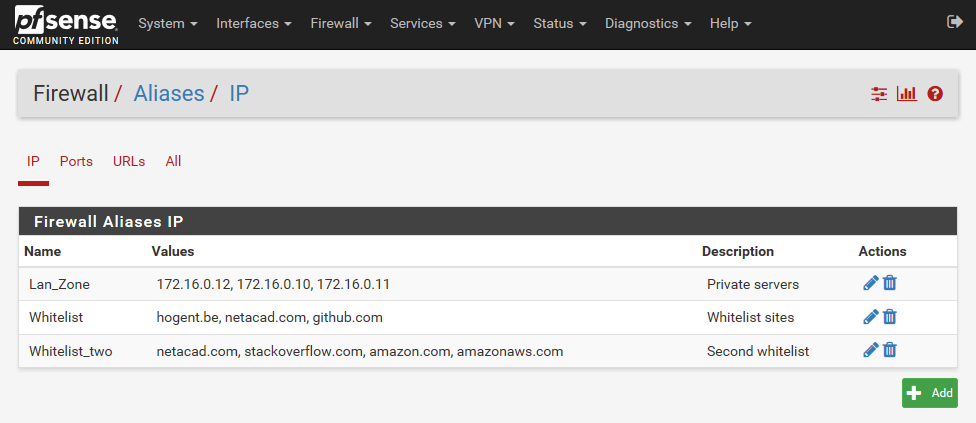
\includegraphics[width=\textwidth]{img/Pfsense_Alias.png}

The aliases used here are:
\begin{itemize}
\item LAN\textunderscore Zone: The local servers, these are not used in any rules here but just serve as an example.
\item Whitelist: This list contains certain sites that we want to reach. On this list the option ``Type`` was set to Host(s). This requires you to fill in an IP-Address or a Fully qualified domain name. In this list there are some websites that we want to reach.
\item Whitelist\textunderscore two: This list has the same purpose as the list above it but here the option was set to Network(s). This requires you to fill in addresses in CIDR format. But if you set the subnet mask to /32 you of course can still specify a single IP address. Both these options were chosen just to show that both work. Again in this list are some websites that we want to access.
\end{itemize}
When adding a list, a name has to be chosen. This name should be a logical one as this has be used as a reference. The remaining settings are quite straight-forward and  can be set to your own choosing.
There is also a possibility to add port and url groups. But as the IP setting fulfills our needs we won't use these. Nevertheless, as the name suggests, these are used to make aliases for groups of ports and urls. (As you may have noticed this is very similiar to the groups configured on a Vyos router).
When all the desired aliases have been set the next step should be configuring the rules. The rules that were set in this example are:

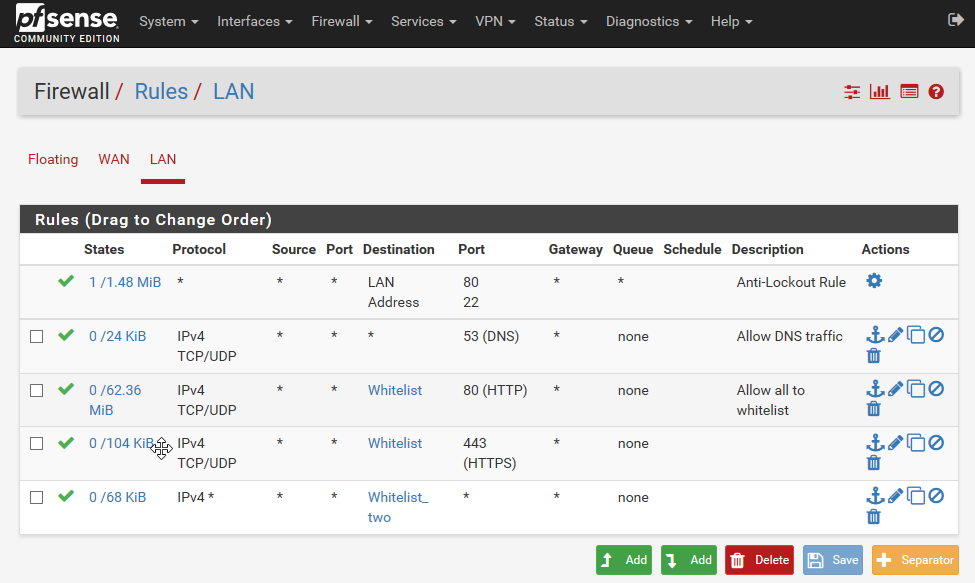
\includegraphics[width=\textwidth]{img/Pfsense_Rules.png}
\begin{itemize}
\item The first rule is added automatically by PfSense to prevent you from locking yourself out.
\item The second rule allows traffic to DNS servers. As we are not blocking DNS access but rather blocking website access this is important to have. Otherwise no site would work, whitelisted or not.
\item The third rule allows HTTP (port 80) TCP/UDP traffic for the hosts listed on the Whitelist list.  The next line allows HTTPS traffic for the same list of hosts. These combined makes it possible for most sites to load. Although some exceptions might not have enough with these two ports. Further investigation is then required into which ports should be open. When these are known they should be added.
\item The last rules allows all IPv4 traffic to the networks specified in the Whitelist\textunderscore two list. 
\end{itemize}
After this is done, all necessary configurations are made. Everything that is not mentioned in any rule will be dropped. So only access to the sites/domains on our lists are allowed now. Do remember if you are working with local resources to allow these in the rules as well (not mentioned in this screenshot). Otherwise you won't be able to communicate with local servers. This configuration is very quickly done and should have the same effect as router ACL's. \\

But remember the mention of the possibility to have the same functionalities as our DNS whitelist. This can be achieved by using the DNS resolver/forwarder option. If these are enabled one could simply block all DNS traffic going out and add the wanted addresses to the Host/Domain overrides at the bottom of the configuration page. Once this is done the web pages will be accessible again. Do not forget to enable the HTTP/HTTPS traffic though.
\subsection{Effectiveness/conclusion}
Not much new can be said here for the Effectiveness as it does the exact same as our Router ACL or DNS whitelist. Except that it is combined into one web interface. And that is the big obvious pro here. The fact that it is very easy to use. Except for the configuration of the interfaces, no console is required. Everything can be configured with a user interface and a modern and easy to use one. But maybe for some, this might be a downer as it allows inexperienced users to do more damage if they would get it.\\

The only other problem that I noticed while using PFSense is the fact that apparently PFSense (and the Edge browser as well) will sometimes remember certain translations or other data which enables a user to visit sites that were visited when certain rules were not enabled yet. This can be prevented when certain options are disabled though, most of these can be found under the advanced tab. A general problem with the previous three tested methods is the fact that it's not always easy to find out what ip/protocol/domain to allow to be able to reach certain websites.\\

 The ``netacad.com`` domain for example would not load while everything was allowed, while other sites on the same list were loading perfectly. It is assumed that this has to do with certain redirection and the site being hosted on addresses that are not the ones that a simple tracert of nslookup will give you. 
\section{Safe Exam Browser}
\subsection{Setting up SEB}
The browser can be downloaded from the official site \footnote{https://www.safeexambrowser.org/download\textunderscore en.html}. The download comes as an .exe file and installs 3 programs. The browser itself, the configuration tool and a Registry Resetter. The resetter is used when certain system changes, that the installation of SEB has done, have interfered with something. Normally this won't happen (in this thesis no problems were encountered) but if it were to happen than this tool will reset all those changes in the windows registry and the system will be back to the state is was before. When uninstalling SEB the system changes won't be undone as well, so it's a good idea to run the resetter before uninstalling the application.\\

Starting the browser without having any configuration set will land you on a standard page that informs the user that no configurations were made. On this page there is information given as to how one has to open SEB using a configuration file or link.
The most important part for us is of course the SEB config tool. This allows the user to personalize our browser to our needs and gives us the ability to create a .seb file which when opened opens up the browser with the correct configurations. As there are quite some options to consider the config tool will be explained in the next section.
\subsection{SEB Config Tool}
The General tab is used as the title suggests to configure the general settings. The link that is pasted in the ``Start URL`` box is the URL on which  the browser will open. So this will be the link that the students need to partake in the examination. In this case it would be \textit{Chamilo.hogent.be} or something alike. The administrative password is the password that is needed when the .seb file wants to be changed. Thus this is a password that needs to be kept secret from students. Otherwise they would obviously be able to change settings to their own liking. The quit/restart password is needed when a users wants to quit the application. It is also a good idea to keep this private. Even though most students won't take the risk of closing their browser during a test (because of the chance that the test will get handed in with their progress so far).\\

The two options left both are concerning the possibilities of closing SEB. Enabling the first one enables the user to close SEB (still requiring the set quit password), when this is not set, no close button is shown. The second option, when disabled, enables a user to close the application using the hot-keys specified to the right. When using these hotkeys no password is requested, thus it is not advised to use this option. A student would have to know the hot-key combination to be able to close the application but when they are really desperate and start smashing all the F-keys chances are that they will hit the correct combination once.\\

The Config File tab includes all settings concerning the configuration file that a student needs to start their SEB browser to take the examination. At least when the first radio button is selected. The second button will configure the client without booting it. This might be useful in some cases when no specific start page is set but there is still need to use SEB as a browser.
The option ``Allow to open preferences window on client (Mac)`` should be disabled as this has no use besides for debugging purposes. The encrypting setting is to encrypt the .seb file. This might be useful if you have certain security concerns. The Settings password makes it so that a student will have to enter a password if he wishes to change the settings in the .seb file. This password should be kept secret as well. The rest of the options are all different actions you can take with the file. Save the file, revert it, use it to perform certain actions.\\

The user interface tab allow for a broad variety of configurations concerning what is shown in the browser once booted. The view mode should probably be set to Full screen mode as this disables a lot of OS functions already ( i.e. the task bar, dragging the window across the screen,...). Audio is of little importance but it might be useful to have it enabled if certain questions or functions require sound. The Mac specific settings should all be disabled as we want users to have as little access to their system as possible.\\

 In the SEB task bar some option can be useful however to be shown. The time is something that is a big help to a lot of students and disables any need for a personal watch (less ways to cheat). The reload button and keyboard layout settings are useful as well as these might always come in handy when something small goes wrong. The remaining options are all to little importance to the security of the application and can be enabled or disabled to your own liking. Except for the dictionary lookup option as this again enables Mac users to use functions that we do not want.\\

The fourth tab has a lot of options but most of them are really depending on the scenario in which the browser is deployed. The first set of options is important to all situations however. Blocking traffic to different servers and opening new tabs should be blocked if this is possible in the specific situation.  It, again, limits the student a lot when they only have the one window to work with, allowing different tabs only increases the chance of them finding ways to opening websites that they should not visit. The remaining options are of little importance here. Just remember to allow the necessary things in the Browser security section if some of these are required for your test to work. But again, be cautious of the options that allow users to open up extra tabs.\\

The download and upload tab can be useful when a student is required to make something in a web browser and has to hand in some result elsewhere (to a file server for instance). The browser is not closed or minimized when downloading a file so an exit password would still be required if a student would attempt to download something that he is not allowed to use. And of course when requesting the password from a teacher, they would decline that request.\\

The Exam tab holds an option that is only useful when using a E-learning platform that is fully integrated with SEB. In this scenario (chamilo) that is not case. This option is the Browser Exam Key. This makes it so that the test only runs when the user is using the correct browser with the correct settings,  which adds a very effective layer of protection. But as it was mentioned, in this scenario we can not use this.\\

 The other links can be filled in to your own liking. In our case no quit link was given and an exit password is required. This gives the teacher the possibility to take a last look at someones screen and to get their signature for instance. It might not be a bad idea either to protect the ``back to Start`` button with the exit password so no student can press it accidentally (or claim that they pressed it accidentally to get certain advantages).\\

The following three tabs (Applications, Additional Resources and network) are all used in situations where a user is allowed more access than just the one tab that they are given when starting up the browser. The application tab allows for third party software to be opened. This of course brings a lot of security issues as some application may have a personal web function installed that would allow students to surf the web (SEB is not able to control what happens inside an other application). The Additional Resources tab allows as the name suggests the use of extra resources.\\

 If some files are allowed during the examination, this is where they could be added (for instance a certain PDF file, a database,...). The network tab allows the filtering of certain URLs. Remember that this only filters URL's inside the SEB browser. So if a user already has no access to other pages, one should not bother with these settings. They can however be useful to filter out certain parts of URLs. For example the location of the images of a web page. When this would be filtered out the webpage would load without images.
When a student is allowed to use other pages however, this can be used as your own personal blacklist of addresses that should not be visited.\\

The Security tab  has some important options that should be enabled/disabled. For instance the option to boot SEB in a virtual machine should always be disabled (not checked) as this would allow students to cheat extremely easily. The service should always be running, this allows SEB to block and allow certain OS functions. When this would be disabled a lot of functions would not work and once again, a loophole for cheating would be created. The Mac options should be disabled as well and logging can be enabled. It doesn't really hurt anyone and can be useful in situations where there is doubt about someones activities. The kiosk mode determines how third party applications that are allowed are booted. The ``Create new desktop`` option is  the safest choice here.\\

The two remaining tabs contain options that one should decide for their own if they should be disabled or not. Be careful however to not allow to much but also to not allow to little. In the making of this thesis no options in the entire config tool were selected concerning closing down the application, which resulted in a computer that had SEB running and was not able to be closed down/logged out / shut down except for forcing it to shut down using the physical shut down button. This is not a situation you would want to find yourself in.\\

After these settings were all configured the config.seb file can be downloaded. This is then used to start up the browser which will show you the start page that was selected. When booting however the configuration password is requested twice, so make sure that this password is secure and not forgotten or you will be locked out of the file (as configuring it requires the same password).
\subsection{Effectiveness/conclusion}
The all-round experience with SEB has been excellent. This application allows protection on a whole new level compared to the previous tested methods. Not only does it secure access to web pages and the internet in general but it also controls access to the system itself without anyone of the school having to configure students personal computers (which would probably cause  privacy issues).\\

The only problem that might pop up is when using a LSM that has no integrated support for SEB so there is no way to check if a student is actually using the SEB browser except for actually looking at their screen. A solution to this would be to keep the config password secret and have the overseer/teacher fill it in every computer in the room. This way when the password does not work, they know that the student is trying to use a self configured version of the SEB browser. Or if a student simply does not request the password they already know that something is wrong. This combined with setting an exit password enables the overseer to have full control of the students activity. Once SEB is started it should not be closed until the exam is finished and thus the exit password should not be given out before this is the case.


%\input{...}
%\input{...}
%...

%%=============================================================================
%% Conclusie
%%=============================================================================

\chapter{Conclusion}
\label{ch:conclusie}

%% TODO: Trek een duidelijke conclusie, in de vorm van een antwoord op de
%% onderzoeksvra(a)g(en). Wat was jouw bijdrage aan het onderzoeksdomein en
%% hoe biedt dit meerwaarde aan het vakgebied/doelgroep? Reflecteer kritisch
%% over het resultaat. Had je deze uitkomst verwacht? Zijn er zaken die nog
%% niet duidelijk zijn? Heeft het onderzoek geleid tot nieuwe vragen die
%% uitnodigen tot verder onderzoek?

\section{Comparing the different methods}
The obivous winner of these methods is SEB. It is extremely easy to implement, blocks traffic on way more levels than the other methods do and is very user friendly. And with the correct handling it could be quite unbreakable for students. It is amazing that a tool like this is not being used more frequently. The biggest reason for this is probably because a lot of people simply do not know that it exists. But as big contributors to this software are mostly located in countries who are leading in education worldwide it might not be a bad idea to pick this up.
Upon discovery of this tool the other methods kind off faded in importance and usefulness. As all the other methods only really tackle one issue in the wide range of cheating possibilities. But from the other tested methods DNS whitelisting seems to be the worst one. It has the most loopholes and is harder to implement than the other two are. As well as it has a bigger impact on the network. If a local DNS is already present there will have to be made quite some changes to the configuration. As well as the difficulty  of adding all the IP's and domain names to list. One might argue that a blacklist might be better because there are often offered online. But these will always be one step behind. It's easier to find a certain fish in a lake when only 6 fish are swimming in it, than it is in an ocean where millions of fish are swimming even though a few million have already been pulled out.\\
The ACL's and the firewall are on the same level. If one of these two would be chosen, it's really a matter of preference. The firewall allow for great configuration that goes way farther than simply filtering traffic. But it is once again an extra device that is needed. While a router is present in the network and can do the same functions that are required without having to spend anything new on equipment.  Plus in this thesis the configuration of the router went a lot smoother than the firewall. This can of course depend from system to system, which is way the choice between these really depends on the situation one is in. Both get the job done though. They are a lot easier to implement than DNS whitelisting is. They are more tightly sealed and are more difficult to trick.\\
So all around SEB is the overall winner with ACL's and firewall on a shared second place. A combination of the both could be used as well of course. When certain exams require specific multiple websites to be accessible SEB could be used to prevent the student from using any local documentation while an ACL could block the websites that are not allowed. Doing this one creates a flexible,dynamic and multi functional network in which exams can be made safely.
\section{Issues with the tested methods}
The biggest issue was the fact that a lot of these methods count on the IP or the full qualified domain name of a website. While this is not always as easy to get. A lot of (probably almost all) websites these days using multiple third party components to host their site. This means that simply allowing or blocking one IP-Address / FQDN does not do the trick. When we want to allow a website it might nog load completely or just refuse to load because of certain rules. And when blocking one it might still be accessible to some extend. Figuring out all the information needed to allow one website can be a lot of work and cause a lot of headaches. Furthermore, when the required information is found it might lead to a server on which multiple websites are stored. Trying to block that one website can be very irritating as these websites might change IP's which would lead to us blocking and allowing the wrong sites. Which of course is not in our interest.\\
An other exploit that might come to mind is the use of VPN's. These however could be blocked by blocking certain ports using a firewall/ACL's (which gives these an other advantage above DNS whitelisting). These ports might be quite big in numbers. But they could all be added to a single port group and then added to the block list whenever an exam is conducted. This way no VPN's would be possible but some other functions might malfunction as well at the same time (for some VPN systems for instance once would have to block the SSH port).\\
The last small issue is the fact that Chamillo was not a LSM that is integrated with SEB which limited the testing possibilities. Even though the system is pretty great with a not integrated LSM, it's always good to improve. Maybe someday the Chamillo community will take a look at this and integrate SEB.
\section{Concerns outside of the general environment}
A brief mention should be made to remind people that all the above methods can be made obsolete by some stupid mistakes. If a student manages to use his smartphone all walls are down again. The same goes with god old fashioned cheating using pen and paper. These systems should of course still be prevented by for instance collecting the phones at the start of an examination and handing them back after it. And using only see through pen cases or no pen cases at all. Equally harmful would be an uninformed teacher/overseer. If a student would be able to trick a teacher into giving them information that he should not know, just because the teacher is not someone with great IT knowledge, the whole system once again topples over. To prevent this all teachers and overseers should always be told the information they need. And to not share this information with anyone. Or call someone with the required knowledge when a problem occurs.
\section{Answering the research questions}
\subsubsection{Can we limit access to the internet to only the necessary item?}
A question that is not easily answered. But after this thesis the answer would be yes. Even though students will probably always find a way to circumvent the systems. At the time of deployment there is a possibility to make environments in which only access is given to the required resources. This can be done by using SEB, or ACL's or a combination of the both. While still taking in account the rules outside of the digital world of course (as mentioned in \textit{5.3}.
\subsubsection{Is it possible to set up an exam server, which is only accessible to registered students, where the exams are submitted digitally?}
Even though this question was not anywhere in the spotlight in this thesis, it was mentioned sometimes. The methods still allow all internal servers to be accessed. This was tested by a file server in the test environment. This file server had a share that could be accessed by teachers only, by teachers and students but students could only upload files and a folder in which students could only download. This all stays functional of course after the implementation of the methods as these methods only act on traffic that is willing to leave the traffic. As long as it stays locally nothing will happen to it.
\subsubsection{Can personal applications be filtered while allowing certain necessary programs?}
Yes, as mentioned in the section about SEB, this has functions available exactly for that. There might be other ways possible but research into these seems pointless as SEB does a great job in this.
\subsubsection{Can the setup of this environment be automated so every teacher can easily set up his own exam room?}
Yes. In the part about automation the more technical side was approached \textit{(2.2)}. But once all the necessary files have been created (scripts,roles,conf.seb files) the process becomes pretty easy .With a short and simple explanation most people would probably be able to execute the automation themselves.
\subsubsection{Can this all be done with currently available technology or should the school invest in new equipment/software?}
It depends. If the school wants to use old equipment it would of course work. Nothing that was described in this thesis needs new devices. But maybe in some situations it might be useful to have seperate devices with each it's function. For instance one exam router and one all-round router. This would only require the switch of a cable to implement a whole other system. SEB does not require any new technology whatsoever though. And is supported by all generally used operating systems. Which results in a very low cost implementation.
\section{Possibility for further research}
The integration of SEB into Chamillo would be interesting to further investigate. It make the lives of the teachers a lot easier in our school. Maybe it can be made so that SEB is actually installed on a server in the school and that the students boot it via that server and this way it might add an extra layer of protection. Research around the other methods seems kind of a waste of time as it is clear that there are way more modern and better choices on the market that do much more. The only things that might be interesting is to find a way to effectively find correct IP addresses for certain domains which you want to block that keeps being up to date. So basically, automating the setup of a dynamic whitelist. 

%%=============================================================================
%% Bijlagen
%%=============================================================================

\appendix

%%---------- Onderzoeksvoorstel -----------------------------------------------

\chapter{Research proposal}

The subject of this thesis was based on the research proposal that was evaluated beforehand by the promotor. The proposal is added in this attachment.

% Verwijzing naar het bestand met de inhoud van het onderzoeksvoorstel
%---------- Inleiding ---------------------------------------------------------

\section{Introduction} % The \section*{} command stops section numbering
\label{sec:introductie}

Students sometimes have to take an exam digitally at the University College of Ghent. This now happens on PCs provided by the college in computer classrooms. However, this is something we want to get rid of. If students always have the opportunity to take exams and tests via their own computers, this will provide more freedom for both the school and the students. More exams can be taken digitally and the amount of digital examinations that are taken simultaneously can be increased. This no longer depends on the number of computer classrooms that are available.\\
\\
\\
The system now allows you to take digital exams, but not in optimal conditions. Currently there is a big possibility of cheating during an exam. Students use the internet while this is not allowed, communicate with each other or use prohibited applications. Completely removing internet access in the classrooms is now possible (by simply disconnecting the classroom from the school network) but is not wanted in a lot of cases. If we implement an exam server access to the network must be possible. Exams which require logging  into external sites (e.g. netacad) require internet access as well.  With no immediate changes in sight, more teachers tend to take a step back and take written examinations. The exact opposite of what is desired. However, neither the students nor the teachers are to blame but the system is. We want to succeed in designing a system, where fraud is eliminated and students can use their own laptop to take the exams. Setting up these environments should be automated so that this can be done quickly and flexibly. For example, dozens of ordinary classrooms can suddenly serve as computer classrooms. \\
\begin{itemize}
  \item \textbf{Goal}: Creating an environment in which we are able to conduct a digital exam while limiting the possibilities to cheat.
  \item \textbf{Research questions}:
\begin{itemize}
   \item Can we limit access to the Internet to only the necessary items? (e.g. allowing access to chamillo.hogent.be / netacad.com but not YouTube / Google )
   \item Is it possible to set up an exam server, which is only accessible to registered students, where all the exams are submitted digitally?
   \item Can personal applications be filtered while allowing certain necessary programs?
   \item Can the setup of this environment be automated so every teacher can easily set up his own exam room?
   \item Can this all be done with currently available technology or should the school invest in new equipment/software?
  \end{itemize}
\end{itemize}

%---------- Stand van zaken ---------------------------------------------------

\section{State-of-the-art}
\label{sec:state-of-the-art}

\subsection{At the University College of Ghent}
At the University College of Ghent there are computer classrooms filled with desktops. These all have the required applications installed that are required for taking tests and/or exams. The access to the internet or certain applications is currently limited by the use of NetOp. Some exams require a teacher to be able to use such a classroom. But this puts a limitation on the amount of digital exams that can be taken at one time. This limit being equal to the amount of available computer classrooms. If teachers are brave enough to allow students to take an exam on their personal devices then the chance of fraud rises exponentially. 
\\
\subsection{At the Brunel University London}
By reading the\emph{ Digital Assessment Blog} by the Brunel University of London ~\autocite{Brunel2017} we can see that other schools are trying the same thing. Here we find that they had issues as well. Their issues are not related to cheating though. The main issues they are describing is the loss of power or internet connections. These are factors that we did not account for thus far. But I believe that our system is small enough to not have these kind of problems. \\
An other issue they describe is the fact that not all students own a personal device and have to rely on the school computer system. But in our case laptops are a must have so this issue won’t come up as much. And if it does, maybe we can configure some current desktops to work with the new environment we would build. \\

\subsection{Cheating at Digital Exams}
\emph{Aleksander Heintz} wrote his thesis on the subject of Cheating at Digital exams, Vulnerabilities and Countermeasures \autocite {Heintz2017}. He researches the way students can cheat at BYOD exams on his university. Even though his research is quite specific to their situation, he still has some interesting points. His conclusions say that there will always be ways to cheat though. Even though people will keep working on finding new ways of solving certain exploits or loop holes that students find. The students will always find a way to sidestep these solutions. But it will get harder and harder for students to do so, and so maybe we will reach a point on which it is easier for a student to just learn for the exam instead of going through a lot of trouble to cheat his way through.

%---------- Methodologie ------------------------------------------------------
\section{Methodology}
\label{sec:methodologie}

Building a virtual network to mimic the desired situation will be a big part of the Methodology. This will be realised by using software like virtual box and Cisco Packet Tracer. Using this we'll be able to get a good idea of the desired configuration of all the devices (servers, clients, routers, ... ).

%---------- Verwachte resultaten ----------------------------------------------
\section{Expected Results}
\label{sec:verwachte_resultaten}

We expect to find a configuration for the network to limit the access to the internet. This will probably be for a Wireless Access Point (WAP). A file consisting out of configuring multiple access-lists, security settings, etc. \\
A fully configured exam server is another result we'll expect. This may be physical or virtual using the most suited OS (a Windows version or a Linux distribution). Access to the server will be limited to certain students and the files will be sufficiently protected. The specific use of the exam server is not clear yet. It could be a simple server from which the students can download their exams and then upload them again. This is the simplest version that we can expect. But maybe other uses can be found for it. For example: making it the only accessible server on the network and hosting software on there which students can use to complete the exam. Make a service that randomises all possible questions and makes an unique exam for each student. But these are extra’s that may not come to be discussed during this bachelor thesis. 
\\
Automating the setup will depend of what OS is used for the exam server. If it's Linux based this will be an Ansible role. If it's Windows based it will be more difficult but doable with shell scripting, using software like chocolatey and general Windows Automation features. \\


%---------- Verwachte conclusies ----------------------------------------------
\section{Expected conclusions}
\label{sec:verwachte_conclusies}

Students will be able to partake in an digital exam using their own devices. The possibility to cheat will be eliminated by using a combination of techniques. This way students and teachers will have an easier way of taking examinations. Students will be comfortable with their own device. Teachers won’t have to worry about possible cheaters because this responsibility will be taken away from them. \\
This will be realized by using a configured WAP or a similar network device that limits the access for students partaking in the examinations. The exams will be handed into a pre-configured exam server. This server is secure as well.  Meaning that students will only be able to hand in their exams during the period that it’s allowed and won’t be able to change it once it’s handed in. \\
The cost of implementing a system like this will be minimized by automating as much as possible. This way implementation is quick and easy. And if additional servers/devices need configuring the same automatization can be used.\\




%%---------- Andere bijlagen --------------------------------------------------
% TODO: Voeg hier eventuele andere bijlagen toe
\label{ch:bijlagen}

\newpage
\begin{lstlisting}[
frame=single,
breaklines=true,
caption=VagrantFile,
language=Ruby,
basicstyle=\ttfamily,
keywordstyle=\color{red},
stringstyle=\color{blue},
]
# -*- mode: ruby -*-
# vi: ft=ruby :

require 'rbconfig'
require 'yaml'

# Set your default base box here
DEFAULT_BASE_BOX = 'bento/centos-7.4'

VAGRANTFILE_API_VERSION = '2'
PROJECT_NAME = '/' + File.basename(Dir.getwd)

# When set to `true`, Ansible will be forced to be run locally on the VM
# instead of from the host machine (provided Ansible is installed).
FORCE_LOCAL_RUN = false

$ITERATIONS = 0
hosts = YAML.load_file('vagrant-hosts.yml')

# {{{ Helper functions
def provision_ansible(config)

  if run_locally?
    # Provisioning configuration for shell script.
    #The Iteration is here to prevent the provisioning from looping, as the command is being called inside a loop this stops it from being executed every call.
    if $ITERATIONS == 0
    config.vm.provision 'shell' do |sh|
      sh.path = 'scripts/playbook-win.sh'
    $ITERATIONS = 1
    end
  end
  else
    # Provisioning configuration for Ansible (for Mac/Linux hosts).
    config.vm.provision 'ansible' do |ansible|
      ansible.playbook = 'ansible/site.yml'
      ansible.sudo = true
    end
  end
end

def run_locally?
  windows_host? || FORCE_LOCAL_RUN
end

def windows_host?
  RbConfig::CONFIG['host_os'] =~ /mswin|mingw|cygwin/
end

# Set options for the network interface configuration. All values are
# optional, and can include:
# - ip (default = DHCP)
# - netmask (default value = 255.255.255.0
# - mac
# - auto_config (if false, Vagrant will not configure this network interface
# - intnet (if true, an internal network adapter will be created instead of a
#   host-only adapter)
def network_options(host)
  options = {}

  if host.key?('ip')
    options[:ip] = host['ip']
    options[:netmask] = host['netmask'] ||= '255.255.255.0'
  else
    options[:type] = 'dhcp'
  end

  options[:mac] = host['mac'].gsub(/[-:]/, '') if host.key?('mac')
  options[:auto_config] = host['auto_config'] if host.key?('auto_config')
  options[:virtualbox__intnet] = true if host.key?('intnet') && host['intnet']
  options
end

def custom_synced_folders(vm, host)
  return unless host.key?('synced_folders')
  folders = host['synced_folders']

  folders.each do |folder|
    vm.synced_folder folder['src'], folder['dest'], folder['options']
  end
end

# }}}

Vagrant.configure(VAGRANTFILE_API_VERSION) do |config|
  config.ssh.insert_key = false
#   VyOS Router, comment line 89-104 if you want the PFSense router/Firewall to be build.
#  config.vm.define 'router' do |router|
#    router.vm.box = 'bertvv/vyos116'
#    router.vm.network :private_network,
#      ip: '192.0.2.254',
#      netmask: '255.255.255.0',
#      auto_config: false
#    router.vm.network :private_network,
#      ip: '172.16.255.254',
#      netmask: '255.255.0.0',
#      auto_config: false
#    router.ssh.insert_key = false

#    router.vm.provision "shell" do |sh|
#      sh.path = "scripts/router-config.sh"
#    end
#  end
  #PFSense firewall, comment line 106 -  127 If you want the VYoS router to be build.
  config.vm.define 'firewall' do |firewall|
    firewall.vm.box = 'kennyl/pfsense'
    firewall.ssh.username = 'vagrant'
    firewall.ssh.password = 'vagrant'
    firewall.ssh.shell = '/bin/sh'
    firewall.vm.guest = 'freebsd'
    firewall.vm.synced_folder ".", "/vagrant", disabled: true
    firewall.vm.network :private_network,
      ip: '172.16.255.254',
      netmask: '255.255.0.0',
      auto_config: false
    firewall.ssh.insert_key = false

    firewall.vm.provision "file" do |fil|
      fil.source = "scripts/FirewallScript"
      fil.destination = "/home/vagrant/"
    end
    
    firewall.vm.provision "shell" do |sh|
      sh.path = "scripts/FirewallScript/firewall-config.sh"
    end
  end
  hosts.each do |host|
    config.vm.define host['name'] do |node|
      node.vm.box = host['box'] ||= DEFAULT_BASE_BOX
      node.vm.box_url = host['box_url'] if host.key? 'box_url'

      node.vm.hostname = host['name']
      node.vm.network :private_network, network_options(host)
      custom_synced_folders(node.vm, host)

      node.vm.provider :virtualbox do |vb|
        # WARNING: if the name of the current directory is the same as the
        # host name, this will fail.
        vb.customize ['modifyvm', :id, '--groups', PROJECT_NAME]
        vb.memory = 512
      end
      #This function is placed inside this loop to prevent it from being called on the router and firewall
      provision_ansible(config)
    end
  end
end
\end{lstlisting}

\newpage


\begin{lstlisting}[
frame=single,
breaklines=true,
caption=Vagrant-hosts.yml,
language=Ruby,
basicstyle=\ttfamily,
keywordstyle=\color{red},
stringstyle=\color{blue},
]
# vagrant_hosts.yml
#
# List of hosts to be created by Vagrant. This file controls the Vagrant
# settings, specifically host name and network settings. You should at least
# have a `name:`.

---
- name: samba
ip: 172.16.0.11
netmask: 255.255.0.0

- name: dns
ip: 172.16.0.10
netmask: 255.255.0.0

- name: dhcp
ip: 172.16.0.12
netmask: 255.255.0.0


\end{lstlisting}
\begin{lstlisting}[
frame=single,
breaklines=true,
caption=site.yml,
language=Ruby,
basicstyle=\ttfamily,
keywordstyle=\color{red},
stringstyle=\color{blue},
]
# site.yml
---
- hosts: all
become: true
roles:
- bertvv.rh-base

- hosts: dns
become: true
roles:
- bertvv.bind

- hosts: dhcp
become: true
roles:
- bertvv.dhcp

- hosts: samba
become: true
roles:
- bertvv.samba
- bertvv.vsftpd
post_tasks:
- name: teachers all access in ExaminationFiles
acl:
path: /srv/shares/ExaminationFiles
entity: teachers
etype: group
permissions: rwx
state: present
default: yes
- name: students read access in ExaminationFiles
acl:
path: /srv/shares/ExaminationFiles
entity: students
etype: group
permissions: rx
state: present
default: yes
- name: students prohibit access in Teachers folder
acl:
path: /srv/shares/Teachers
entity: students
etype: group
permissions: ---
state: present
default: yes

\end{lstlisting}
\begin{lstlisting}[
frame=single,
breaklines=true,
caption='group\textunderscore vars/all.yml',
language=Ruby,
basicstyle=\ttfamily,
keywordstyle=\color{red},
stringstyle=\color{blue},
]
# group_vars/all.yml
# Variables visible to all nodes
---

rhbase_install_packages:
- bash-completion
- bind-utils
- git
- nano
- tree
- vim-enhanced
- wget
rhbase_users:
- name: kjell
comment: 'kjell admin'
groups:
- users
- wheel
password: 'KEY'

rhbase_motd: true
rhbase_ssh_user: kjell
rhbase_ssh_key: ssh-rsa SSH

\end{lstlisting}
\begin{lstlisting}[
frame=single,
breaklines=true,
caption=dhcp.yml,
language=Ruby,
basicstyle=\ttfamily,
keywordstyle=\color{red},
stringstyle=\color{blue},
]
# host_vars/pu001.yml
# Variables visible to pr001
---
rhbase_firewall_allow_services:
- dhcp

dhcp_global_authoritative: authoritative
dhcp_global_default_lease_time: 43200
dhcp_global_domain_name: example.lan
dhcp_global_routers: 172.16.255.254
dhcp_global_domain_name_servers:
- 172.16.255.254
dhcp_global_classes:
- name: vbox
match: 'match if binary-to-ascii(16,8,":",substring(hardware, 1, 3)) = "8:0:27"'
- name: reserved
match: 'match if hardware = 1:00:11:22:33:44:55'

dhcp_subnets:
- ip: 172.16.0.0
netmask: 255.255.0.0
pools:
- range_begin: 172.16.0.2
range_end: 172.16.127.254
- range_begin: 172.16.128.1
range_end: 172.16.191.254
allow: 'members of "reserved"'
- range_begin: 172.16.192.1
range_end: 172.16.255.253
allow: 'members of "vbox"'

\end{lstlisting}
\begin{lstlisting}[
frame=single,
breaklines=true,
caption=dns.yml,
language=Ruby,
basicstyle=\ttfamily,
keywordstyle=\color{red},
stringstyle=\color{blue},
]
rhbase_firewall_allow_services:
- dns
bind_zone_master_server_ip: 172.16.0.10

bind_zone_name: example.lan
bind_zone_networks:
- '172.16.0'
bind_zone_name_servers:
- dns
bind_zone_hosts	:
- name: dns
ip: 172.16.0.10
aliases:
- nameserver
- name: samba
ip: 172.16.0.11
aliases:
- files
- name: dhcp
ip: 172.16.0.12
aliases:
- internal

bind_listen_ipv4:
- any
bind_allow_query:
- any
bind_forwarders:
- '172.16.0.10'

\end{lstlisting}
\begin{lstlisting}[
frame=single,
breaklines=true,
caption=samba.yml,
language=Ruby,
basicstyle=\ttfamily,
keywordstyle=\color{red},
stringstyle=\color{blue},
]
rhbase_firewall_allow_services:
- samba
- ftp
rhbase_user_groups:
- students
- teachers
- it
- public

rhbase_users:
- name: kjell
comment: 'kjell admin'
groups:
- wheel
- it
- public
password: 'KEY'
- name: docent
comment: 'docent'
groups:
- public
- teachers
password: 'KEY'
- name: student
comment: 'student'
groups:
- public
- students
password: 'KEY'
shell: /sbin/nologin
- name: student2
comment: 'student2'
groups:
- public
- students
password: 'KEY'
shell: /sbin/nologin
samba_users:
- name: kjell
password: test
- name: docent
password: teacher
- name: student
password: student
samba_shares:
- name: HandIn
comment: 'Share folder to hand in examinations'
group: public
valid_users: +students,+teachers,+it
write_list: +students,+teachers,+it
create_mode: '1775'
force_create_mode: '1775'
directory_mode: '1775'
force_directory_mode : '1775'
- name: ExaminationFiles
comment: 'Share folder where students can find the exams'
group: public
valid_users: +students,+teachers,+it,+public
write_list: +teachers
create_mode: '0775'
force_create_mode: '0775'
directory_mode: '0775'
force_directory_mode : '0775'

- name: Teachers
comment: 'Share folder for teachers, files with account info etc.'
group: teachers
valid_users: +teachers,+it
write_list: +teachers,+it
#directory_mode: '770'
samba_workgroup: example
samba_netbios_name: EXAMINATION
samba_load_homes: true
sambe_load_printers: false
vsftpd_anonymous_enable: false
vsftpd_local_enable: true
vsftpd_write_enable: true
vsftpd_local_umask: '007'
vsftpd_local_root: '/srv/shares/'
\end{lstlisting}
\begin{lstlisting}[
frame=single,
breaklines=true,
caption=inventory.py,
language=Ruby,
basicstyle=\ttfamily,
keywordstyle=\color{red},
stringstyle=\color{blue},
]
#! /usr/bin/python
# coding=utf8
#
# Inventory script for Ansible skeleton, to be used on Windows host systems

import socket
import sys
from getopt import getopt, GetoptError


#
# Helper functions
#


def usage():
print ("Usage: %s [OPTION]\n"
"  --list  list all hosts\n"
"  --host=HOST  gives extra info"
"about the specified host\n") % sys.argv[0]


def list_hosts():
host_name = socket.gethostname()
print "{ \"all\": { \"hosts\": [\"%s\"] } }" % host_name


def host_info(host):
print "{}"

#
# Parse command line
#

try:
opts, args = getopt(sys.argv[1:], "lh:", ['list', 'host='])
except GetoptError as err:
print str(err)
usage()
sys.exit(2)

for opt, opt_arg in opts:
if opt in ('-l', '--list'):
list_hosts()
sys.exit(0)
if opt in ('-h', '--host'):
host_info(opt_arg)
else:
assert False, "unhandled option: %s" % opt

\end{lstlisting}
\begin{lstlisting}[
frame=single,
breaklines=true,
caption=playbook-win.sh,
language=Ruby,
basicstyle=\ttfamily,
keywordstyle=\color{red},
stringstyle=\color{blue},
]
#!/bin/bash
# Source: https://github.com/geerlingguy/JJG-Ansible-Windows/blob/master/windows.sh

# Windows shell provisioner for Ansible playbooks, based on KSid's
# windows-vagrant-ansible: https://github.com/KSid/windows-vagrant-ansible
#
# @todo - Allow proxy configuration to be passed in via Vagrantfile config.
#
# @see README.md
# @author Jeff Geerling, 2014
# @version 1.0
#

#
# Bash shell settings: exit on failing commands, unbound variables
#
set -o errexit
set -o nounset
set -o pipefail

#
# Variables
#
ITERATIONS=0
# Color definitions
readonly reset='\e[0m'
readonly red='\e[0;31m'
readonly yellow='\e[0;33m'
readonly cyan='\e[0;36m'

readonly playbook=/vagrant/ansible/site.yml
readonly inventory=/vagrant/scripts/inventory.py

#
# Functions
#

main() {
info "Running Playbook"
if [ "$ITERATIONS" == 0 ]; then
info "Running Ansible playbook ${playbook} locally on host ${HOSTNAME}."

exit_on_vyos
check_if_playbook_exists
check_if_inventory_exists
ensure_ansible_installed
run_playbook "${@}"
fi
ITERATIONS=1
}

exit_on_vyos() {
# If we're on a VyOS box, this script shouldn't be executed
if user_exists vyos; then
debug "On VyOS, not running Ansible here"
exit 0
fi
}

check_if_playbook_exists() {
if [ ! -f ${playbook} ]; then
die "Cannot find Ansible playbook ${playbook}."
fi
}

check_if_inventory_exists() {
if [ ! -f ${inventory} ]; then
die "Cannot find inventory file ${inventory}."
fi
}

ensure_ansible_installed() {
if ! is_ansible_installed; then
distro=$(get_linux_distribution)
"install_ansible_${distro}" || die "Distribution ${distro} is not supported"
fi

info "Ansible version"
ansible --version
}

is_ansible_installed() {
which ansible-playbook > /dev/null 2>&1
}

run_playbook() {
info "Running the playbook"

# Get absolute path to playbook command
playbook_cmd=$(which ansible-playbook)

set -x
${playbook_cmd} "${playbook}" \
--inventory-file="${inventory}" \
--limit="${HOSTNAME}" \
--extra-vars "is_windows=true" \
--connection=local \
"$@"
set +x
}



# Print the Linux distribution
get_linux_distribution() {

if user_exists vyos; then

echo "vyos"

elif [ -f '/etc/redhat-release' ]; then

# RedHat-based distributions
cut --fields=1 --delimiter=' ' '/etc/redhat-release' \
| tr "[:upper:]" "[:lower:]"

elif [ -f '/etc/lsb-release' ]; then

# Debian-based distributions
grep DISTRIB_ID '/etc/lsb-release' \
| cut --delimiter='=' --fields=2 \
| tr "[:upper:]" "[:lower:]"

fi
}

# Install Ansible on a Fedora system.
# The version in the repos is fairly current, so we'll install that
install_ansible_fedora() {
info "Fedora: installing Ansible from distribution repositories"
dnf -y install ansible
}

# Install Ansible on a CentOS system from EPEL
install_ansible_centos() {
info "CentOS: installing Ansible from the EPEL repository"
yum -y install epel-release
yum -y install ansible
}

# Install Ansible on a recent Ubuntu distribution, from the PPA
install_ansible_ubuntu() {
info "Ubuntu: installing Ansible from PPA"
# Remark: on older Ubuntu versions, it's python-software-properties
apt-get -y install software-properties-common
apt-add-repository -y ppa:ansible/ansible
apt-get -y update
apt-get -y install ansible
}

# Checks if the specified user exists
user_exists() {
user_name="${1}"
getent passwd "${user_name}" > /dev/null
}

# Usage: info [ARG]...
#
# Prints all arguments on the standard output stream
info() {
printf "${yellow}>>> %s${reset}\n" "${*}"
}

# Usage: debug [ARG]...
#
# Prints all arguments on the standard output stream
debug() {
printf "${cyan}### %s${reset}\n" "${*}"
}

# Usage: error [ARG]...
#
# Prints all arguments on the standard error stream
error() {
printf "${red}!!! %s${reset}\n" "${*}" 1>&2
}

# Usage: die MESSAGE
# Prints the specified error message and exits with an error status
die() {
error "${*}"
exit 1
}

main "${@}"

\end{lstlisting}
\begin{lstlisting}[
frame=single,
breaklines=true,
caption=role-deps.sh,
]
#! /usr/bin/env bash
#
# Author: Bert Van Vreckem <bert.vanvreckem@gmail.com>
#
# Install role dependencies. This script is meant to be used in the context of
# ansible-skeleton[1] and ansible-role-skeleton[2].
#
# This script will search ansible/site.yml (or the specified playbook) for
# roles assigned to hosts in the form "user.role". It will then try to install
# them all. If possible, it will use Ansible Galaxy (on Linux, MacOS), but if
# this is not available (e.g. on Windows), it will use Git to clone the latest
# revision.
#
# Remark that this is a very crude technique and especially the Git fallback
# is very brittle. It will download HEAD, and not necessarily the latest
# release of the role. Additionally, the name of the repository is guessed,
# but if it does not exist, the script will fail.
#
# Using ansible-galaxy and a dependencies.yml file is the best method, but
# unavailable on Windows. This script is an effort to have a working
# alternative.
#
# [1] https://github.com/bertvv/ansible-skeleton
# [2] https://github.com/bertvv/ansible-role-skeleton

set -o errexit  # abort on nonzero exitstatus
set -o nounset  # abort on unbound variable

#{{{ Variables
readonly SCRIPT_NAME=$(basename "${0}")

readonly ansible_root=ansible
readonly playbook=${ansible_root}/site.yml
readonly roles_path=${ansible_root}/roles
#}}}

main() {
local dependencies

process_args "${@}"

set_roles_path
select_installer

dependencies="$(find_dependencies)"

for dep in ${dependencies}; do
owner=${dep%%.*}
role=${dep##*.}

if [[ ! -d "${roles_path}/${dep}" ]]; then
${installer} "${owner}" "${role}"
else
echo "+ Skipping ${dep}, seems to be installed already"
fi
done
}

#{{{ Helper functions

# If the default roles path does not exist, try "roles/"
set_roles_path() {
if [ ! -d "${roles_path}" ]; then
if [ -d "${ansible_root}" ]; then
mkdir "${roles_path}"
else
roles_path="roles"
fi
fi
}

# Find dependencies in the specified playbook
find_dependencies() {
grep '    - .*\..*' "${playbook}" \
| cut -c7- \
| grep --invert-match " " \
| sort --unique
}

# Check if command line arguments are valid
process_args() {
if [ "${#}" -gt "1" ]; then
echo "Expected at most 1 argument, got ${#}" >&2
usage
exit 2
elif [ "${#}" -eq "1" ]; then
if [ "${1}" = '-h' ] || [ "${1}" = '--help' ]; then
usage
exit 0
elif [ ! -f "${1}" ]; then
echo "Playbook `${1}` not found." >&2
usage
exit 1
else
playbook="${1}"
fi
elif [ "${#}" -eq "0" ] && [ ! -f "${playbook}" ]; then
cat << _EOF_
Default playbook ${playbook} not found. Maybe you should cd to the
directory above ${playbook%%/*}/, or specify the playbook.
_EOF_
usage
exit 1
fi
}

# Print usage message on stdout
usage() {
cat << _EOF_
Usage: ${SCRIPT_NAME} [PLAYBOOK]

Installs role dependencies found in the specified playbook (or ${playbook}
if none was given).

OPTIONS:

-h, --help  Prints this help message and exits

EXAMPLES:

$ ${SCRIPT_NAME}
$ ${SCRIPT_NAME} test.yml
_EOF_
}


# Usage: select_installer
# Sets the variable `installer`, the function to use when installing roles
# Try to use ansible-galaxy when it is available, and fall back to `git clone`
# when it is not.
select_installer() {
if which ansible-galaxy > /dev/null 2>&1 ; then
installer=install_role_galaxy
else
installer=install_role_git
fi
}

# Usage: is_valid_url URL
# returns 0 if the URL is valid, 22 otherwise
is_valid_url() {
local url=$1

curl --silent --fail "${url}" > /dev/null
}

# Usage: install_role_galaxy OWNER ROLE
install_role_galaxy() {
local owner=$1
local role=$2
ansible-galaxy install --roles-path="${roles_path}" \
"${owner}.${role}"
}

# Usage: install_role_git OWNER ROLE
install_role_git() {
local owner=$1
local role=$2

# First try https://github.com/OWNER/ansible-role-ROLE
local repo="https://github.com/${owner}/ansible-role-${role}"

if is_valid_url "${repo}"; then
git clone "${repo}" "${roles_path}/${owner}.${role}"
else
# If that fails, try https://github.com/OWNER/ansible-ROLE
git clone "https://github.com/${owner}/ansible-${role}" \
"${roles_path}/${owner}.${role}"
fi
}
#}}}

main "${@}"

\end{lstlisting}
\begin{lstlisting}[
frame=single,
breaklines=true,
caption=router-config.sh,
basicstyle=\ttfamily,
keywordstyle=\color{red},
stringstyle=\color{blue},
]
#! /usr/bin/env bash
#
# Author: Bert Van Vreckem <bert.vanvreckem@gmail.com>
#
# Install role dependencies. This script is meant to be used in the context of
# ansible-skeleton[1] and ansible-role-skeleton[2].
#
# This script will search ansible/site.yml (or the specified playbook) for
# roles assigned to hosts in the form "user.role". It will then try to install
# them all. If possible, it will use Ansible Galaxy (on Linux, MacOS), but if
# this is not available (e.g. on Windows), it will use Git to clone the latest
# revision.
#
# Remark that this is a very crude technique and especially the Git fallback
# is very brittle. It will download HEAD, and not necessarily the latest
# release of the role. Additionally, the name of the repository is guessed,
# but if it does not exist, the script will fail.
#
# Using ansible-galaxy and a dependencies.yml file is the best method, but
# unavailable on Windows. This script is an effort to have a working
# alternative.
#
# [1] https://github.com/bertvv/ansible-skeleton
# [2] https://github.com/bertvv/ansible-role-skeleton

set -o errexit  # abort on nonzero exitstatus
set -o nounset  # abort on unbound variable

#{{{ Variables
readonly SCRIPT_NAME=$(basename "${0}")

readonly ansible_root=ansible
readonly playbook=${ansible_root}/site.yml
readonly roles_path=${ansible_root}/roles
#}}}

main() {
local dependencies

process_args "${@}"

set_roles_path
select_installer

dependencies="$(find_dependencies)"

for dep in ${dependencies}; do
owner=${dep%%.*}
role=${dep##*.}

if [[ ! -d "${roles_path}/${dep}" ]]; then
${installer} "${owner}" "${role}"
else
echo "+ Skipping ${dep}, seems to be installed already"
fi
done
}

#{{{ Helper functions

# If the default roles path does not exist, try "roles/"
set_roles_path() {
if [ ! -d "${roles_path}" ]; then
if [ -d "${ansible_root}" ]; then
mkdir "${roles_path}"
else
roles_path="roles"
fi
fi
}

# Find dependencies in the specified playbook
find_dependencies() {
grep '    - .*\..*' "${playbook}" \
| cut -c7- \
| grep --invert-match " " \
| sort --unique
}

# Check if command line arguments are valid
process_args() {
if [ "${#}" -gt "1" ]; then
echo "Expected at most 1 argument, got ${#}" >&2
usage
exit 2
elif [ "${#}" -eq "1" ]; then
if [ "${1}" = '-h' ] || [ "${1}" = '--help' ]; then
usage
exit 0
elif [ ! -f "${1}" ]; then
echo "Playbook `${1}` not found." >&2
usage
exit 1
else
playbook="${1}"
fi
elif [ "${#}" -eq "0" ] && [ ! -f "${playbook}" ]; then
cat << _EOF_
Default playbook ${playbook} not found. Maybe you should cd to the
directory above ${playbook%%/*}/, or specify the playbook.
_EOF_
usage
exit 1
fi
}

# Print usage message on stdout
usage() {
cat << _EOF_
Usage: ${SCRIPT_NAME} [PLAYBOOK]

Installs role dependencies found in the specified playbook (or ${playbook}
if none was given).

OPTIONS:

-h, --help  Prints this help message and exits

EXAMPLES:

$ ${SCRIPT_NAME}
$ ${SCRIPT_NAME} test.yml
_EOF_
}


# Usage: select_installer
# Sets the variable `installer`, the function to use when installing roles
# Try to use ansible-galaxy when it is available, and fall back to `git clone`
# when it is not.
select_installer() {
if which ansible-galaxy > /dev/null 2>&1 ; then
installer=install_role_galaxy
else
installer=install_role_git
fi
}

# Usage: is_valid_url URL
# returns 0 if the URL is valid, 22 otherwise
is_valid_url() {
local url=$1

curl --silent --fail "${url}" > /dev/null
}

# Usage: install_role_galaxy OWNER ROLE
install_role_galaxy() {
local owner=$1
local role=$2
ansible-galaxy install --roles-path="${roles_path}" \
"${owner}.${role}"
}

# Usage: install_role_git OWNER ROLE
install_role_git() {
local owner=$1
local role=$2

# First try https://github.com/OWNER/ansible-role-ROLE
local repo="https://github.com/${owner}/ansible-role-${role}"

if is_valid_url "${repo}"; then
git clone "${repo}" "${roles_path}/${owner}.${role}"
else
# If that fails, try https://github.com/OWNER/ansible-ROLE
git clone "https://github.com/${owner}/ansible-${role}" \
"${roles_path}/${owner}.${role}"
fi
}
#}}}

main "${@}"

\end{lstlisting}
\begin{lstlisting}[
frame=single,
breaklines=true,
caption=firewall-config.sh,
language=Ruby,
basicstyle=\ttfamily,
keywordstyle=\color{red},
stringstyle=\color{blue},
]
#!/bin/sh
pkg install -y git
mv /home/vagrant/FirewallScript/config.xml /cf/conf/
echo "Rebooting now!"
reboot

\end{lstlisting}

%%---------- Referentielijst --------------------------------------------------

\printbibliography[heading=bibintoc]
\addcontentsline{toc}{chapter}{\textcolor{maincolor}{\IfLanguageName{dutch}{Bibliografie}{Bibliography}}}

\end{document}
